\documentclass{article}

% if you need to pass options to natbib, use, e.g.:
\PassOptionsToPackage{numbers, compress}{natbib}
% before loading neurips_2026

% The authors should use one of these tracks.
% Before accepting by the NeurIPS conference, select one of the options below.
% 0. "default" for submission
% \usepackage[eandd]{neurips_2026}
% the "default" option is equal to the "main" option, which is used for the Main Track with double-blind reviewing.
% 1. "main" option is used for the Main Track
%  \usepackage[main]{neurips_2026}
% 2. "position" option is used for the Position Paper Track
%  \usepackage[position]{neurips_2026}
% 3. "eandd" option is used for the Evaluations & Datasets Track
% \usepackage[eandd]{neurips_2026}
% if you need to opt-in for a single-blind submission in the E&D track:
%\usepackage[eandd, nonanonymous]{neurips_2026}
% 4. "creativeai" option is used for the Creative AI Track
%  \usepackage[creativeai]{neurips_2026}
% 5. "sglblindworkshop" option is used for the Workshop with single-blind reviewing
% \usepackage[sglblindworkshop]{neurips_2026}
% 6. "dblblindworkshop" option is used for the Workshop with double-blind reviewing
%  \usepackage[dblblindworkshop]{neurips_2026}

% After being accepted, the authors should add "final" behind the track to compile a camera-ready version.
% 1. Main Track
% \usepackage[main, final]{neurips_2026}
% 2. Position Paper Track
%  \usepackage[position, final]{neurips_2026}
% 3. Evaluations & Datasets Track
% \usepackage[eandd, final]{neurips_2026}
% 4. Creative AI Track
%  \usepackage[creativeai, final]{neurips_2026}
% 5. Workshop with single-blind reviewing
%  \usepackage[sglblindworkshop, final]{neurips_2026}
% 6. Workshop with double-blind reviewing
%  \usepackage[dblblindworkshop, final]{neurips_2026}
% Note. For the workshop paper template, both \title{} and \workshoptitle{} are required, with the former indicating the paper title shown in the title and the latter indicating the workshop title displayed in the footnote.
% For workshops (5., 6.), the authors should add the name of the workshop, "\workshoptitle" command is used to set the workshop title.
% \workshoptitle{WORKSHOP TITLE}

% "preprint" option is used for arXiv or other preprint submissions
\usepackage[preprint]{neurips_2026}

% to avoid loading the natbib package, add option nonatbib:
%    \usepackage[nonatbib]{neurips_2026}

\usepackage{url}            % simple URL typesetting
\usepackage[colorlinks=true,linkcolor=black,citecolor=black,urlcolor=blue]{hyperref}       % hyperlinks
\usepackage{booktabs}       % professional-quality tables
\usepackage{arydshln}       % dashed lines in tables
\usepackage{amsfonts}       % blackboard math symbols
\usepackage{nicefrac}       % compact symbols for 1/2, etc.
\usepackage{microtype}      % microtypography
\usepackage[dvipsnames]{xcolor}         % colors
\usepackage{colortbl}       % table row/cell coloring
\usepackage{graphicx}       % images
\usepackage[most]{tcolorbox} % styled boxes for examples

% dashed rule for separating route options
\newcommand{\dashrule}{\noindent\makebox[\linewidth]{\color{black!40}\dashrulefill}}\newcommand{\dashrulefill}{\leaders\hbox to 5pt{\hss\rule{3pt}{0.4pt}\hss}\hfill}
\usepackage{enumitem}

% Note. For the workshop paper template, both \title{} and \workshoptitle{} are required, with the former indicating the paper title shown in the title and the latter indicating the workshop title displayed in the footnote. 
\title{TransitLM: A Large-Scale Dataset and Benchmark for Map-Free Transit Route Generation}


% The \author macro works with any number of authors. There are two commands
% used to separate the names and addresses of multiple authors: \And and \AND.
%
% Using \And between authors leaves it to LaTeX to determine where to break the
% lines. Using \AND forces a line break at that point. So, if LaTeX puts 3 of 4
% authors names on the first line, and the last on the second line, try using
% \AND instead of \And before the third author name.


\author{%
  Hanyu Guo$^{*}$ \quad Jiedong Yang$^{*}$ \quad Chao Chen \quad Longfei Xu \quad Kaikui Liu \quad Xiangxiang Chu \\[0.5em]
  AMAP, Alibaba Group\\
  Beijing, China\\[0.3em]
  \texttt{\{guohanyu.ghy,jiedong.yjd,cc201598,longfei.xl,damon\}@alibaba-inc.com}\\
  \texttt{cxxgtxy@gmail.com}
}


\begin{document}

\renewcommand{\thefootnote}{*}
%\footnotetext{Equal contribution.}
%\renewcommand{\thefootnote}{\arabic{footnote}}

\maketitle

\begin{abstract}
    Public transit route planning traditionally depends on structured map infrastructure and complex routing engines, and no existing dataset supports training models to bypass this dependency. We present TransitLM, a large-scale dataset of over 13 million transit route planning records from four Chinese cities covering 120,845 stations and 13,666 lines, released as a continual pre-training corpus and benchmark data for three evaluation tasks with complementary metrics. Experiments show that an LLM trained on TransitLM produces structurally valid routes at high accuracy and implicitly grounds arbitrary GPS coordinates to appropriate stations without any explicit mapping. These results demonstrate that transit route planning can be learned entirely from data, enabling end-to-end, map-free route generation directly from origin-destination information. The dataset and benchmark are available at \url{https://huggingface.co/datasets/GD-ML/TransitLM}, with evaluation code at \url{https://github.com/HotTricker/TransitLM}.
\end{abstract}

\section{Introduction}
\label{sec:introduction}
Public transit route planning underpins daily urban mobility, yet conventional systems rely heavily on structured map infrastructure and complex engineering pipelines for candidate retrieval and ranking over topological networks. Notably, massive route planning logs continuously generated by transit platforms implicitly encode rich routing knowledge, including boarding stations, transfer points, and how travelers balance speed, convenience, and line preference. This contrast motivates a natural question: can route planning be learned directly from such data, bypassing maps and routing engines entirely?

One might expect general-purpose LLMs like GPT-3 \cite{brown2020language}, GPT-4 \cite{openai2023gpt4}, and Qwen3 \cite{yang2025qwen3} to address this question with their strong reasoning and broad world knowledge. However, recent studies argue that autoregressive LLMs cannot reliably perform planning by themselves \cite{valmeekam2023planning,kambhampati2024llms}. Although these models may recall frequently mentioned stations or popular routes, they consistently produce routes with hallucinated stations or broken connections \cite{huang2023hallucination}, particularly for less prominent origin-destination pairs. This limitation stems from the absence of suitable training data. Existing data sources each capture only partial aspects of the problem. Vehicle trajectory datasets such as T-Drive \cite{yuan2010tdrive} and Porto Taxi \cite{moreira2013porto} lack station structures. Static network datasets including GTFS \cite{wong2013leveraging} and CPTOND-2025 \cite{wang2026china} contain no user behavior or planning trajectories. Consequently, no existing source provides the complete route structures and behavioral annotations needed for learning end-to-end transit planning.

\begin{figure}[t]
\centering
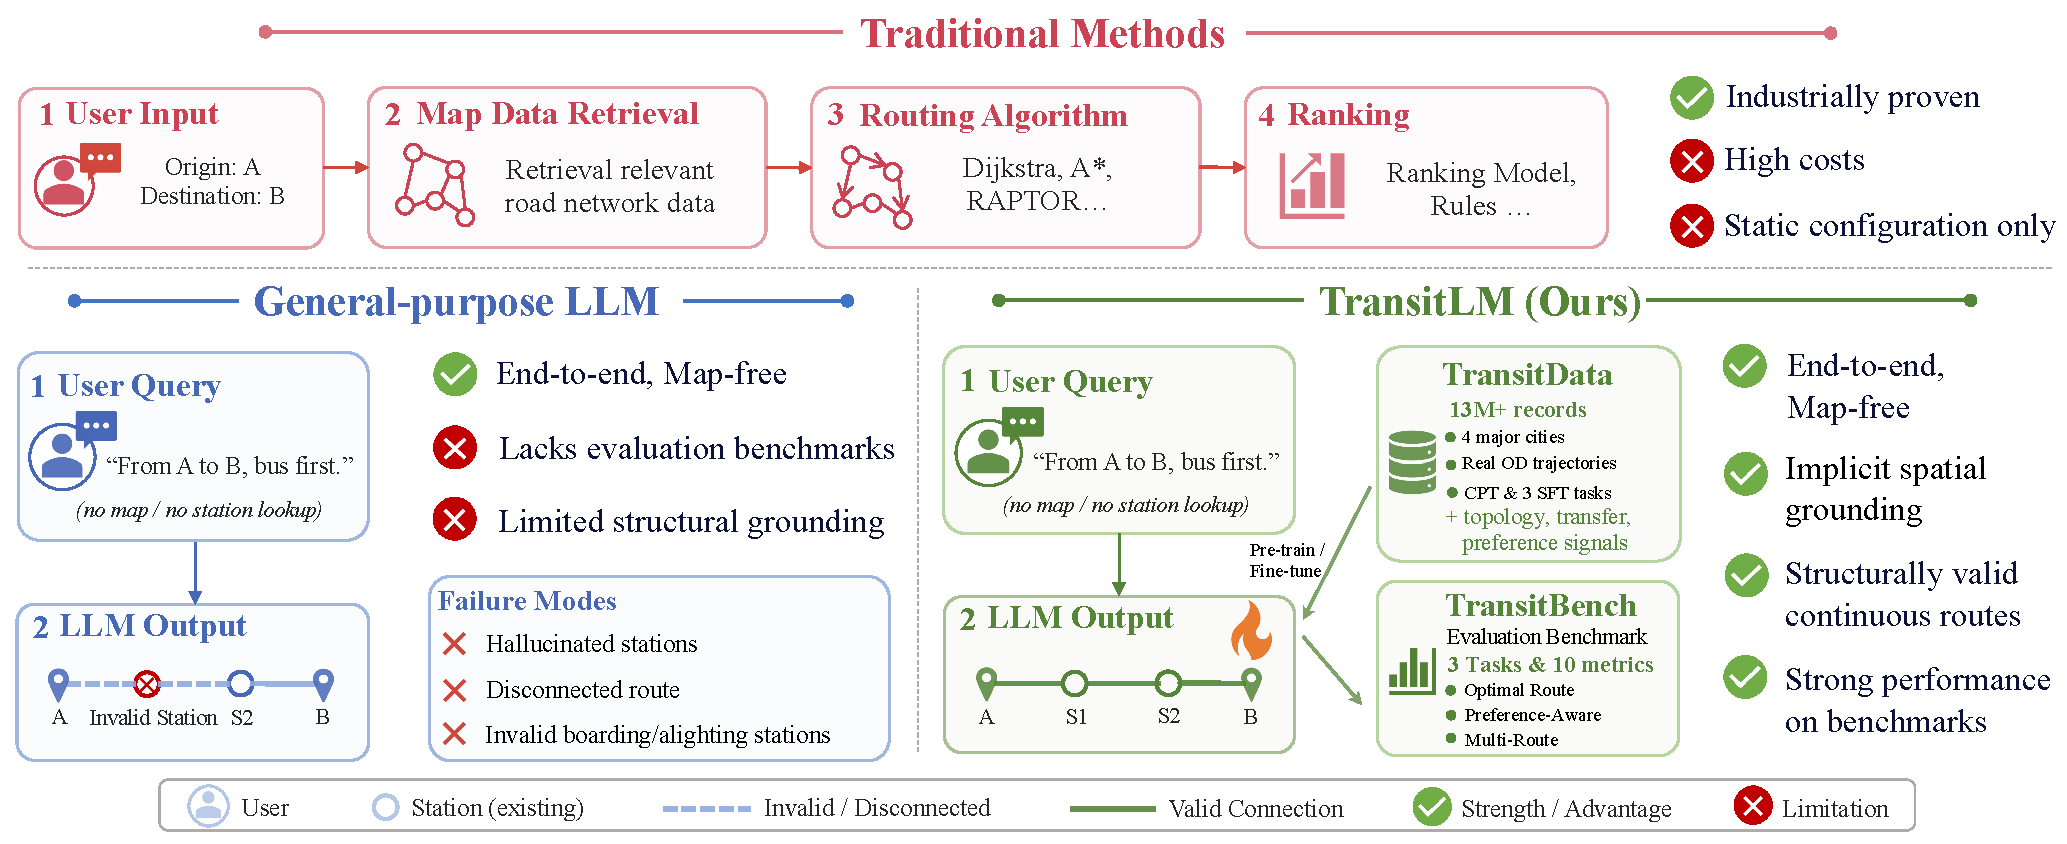
\includegraphics[width=0.96\textwidth]{figures/method_comparison.pdf}
\caption{Three paradigms for transit route planning. \textbf{Top:} Traditional map-based pipeline. \textbf{Bottom-left:} General-purpose LLMs lack structural grounding, producing hallucinated stations, disconnected routes, and invalid boarding/alighting points. \textbf{Bottom-right:} TransitLM generates structurally valid, continuous routes end-to-end via implicit spatial grounding, without map infrastructure.}
\label{fig:method_comparison}
\end{figure}

As illustrated in Figure~\ref{fig:method_comparison}, we introduce TransitLM to address this gap. TransitLM is a large-scale dataset of over 13 million route planning records from four Chinese cities: Beijing, Shanghai, Shenzhen, and Chengdu, covering 120,845 stations and 13,666 transit lines. Each record captures a full planning session with GPS coordinates, station sequences, transfer points, line identifiers, segment-level timing, and route-type annotations. We release two complementary resources. The continual pre-training corpus contains 13.9 million textual route descriptions for next-token prediction training, enabling models to internalize transit network topology and spatial relationships. The benchmark-specific SFT data provides standardized prompts and labels for three core tasks: optimal route generation, preference-aware planning, and multi-route generation, each evaluated by complementary metrics spanning connectivity, access feasibility, route overlap, and numeric field accuracy.

To validate the dataset, we train an LLM through continual pre-training followed by supervised fine-tuning. Our experiments reveal three key findings.
\textbf{(1)~End-to-end map-free route generation is feasible.} The trained model produces structurally valid, connected routes at high accuracy, demonstrating that rich trajectory data alone can replace conventional map-based routing engines.
\textbf{(2)~Implicit spatial grounding emerges from data.} Given only origin and destination GPS coordinates, the model learns to resolve arbitrary coordinates to appropriate boarding and alighting stations without any explicit coordinate-to-station mapping or geographic database, effectively internalizing the spatial topology of the transit network.
\textbf{(3)~A single model generalizes across planning objectives.} A jointly trained model matches or exceeds task-specific counterparts on all three benchmarks without negative transfer, confirming that the transit knowledge encoded in the dataset is task-agnostic and supports unified deployment across diverse planning scenarios.
Our contributions are as follows:
\begin{itemize}[left=0pt]
\item \textbf{Dataset.} We present TransitLM, a large-scale dataset of over 13 million transit route planning records spanning four Chinese cities, 120,845 stations, and 13,666 lines, released as a pre-training corpus and benchmark data with standardized prompts and labels.
\item \textbf{Benchmark.} We define three evaluation tasks: optimal route generation, preference-aware planning, and multi-route generation. Each task is evaluated by complementary metrics spanning connectivity, access feasibility, route overlap, and numeric field accuracy.
\item \textbf{Validation.} We validate the dataset by training an LLM that achieves accurate map-free route generation, exhibits implicit spatial grounding from GPS coordinates to transit stations, and generalizes across diverse planning objectives with a single jointly trained model, confirming that the underlying transit knowledge is task-agnostic.
\end{itemize}

\section{Related Work}

\subsection{Transit Route Planning Methods}

Classical transit routing operates over explicit graph representations. Foundational algorithms such as Dijkstra \cite{dijkstra2022note} and A* \cite{hart1968formal} have been extended by transit-specific methods including RAPTOR \cite{delling2015round} and its Pareto-optimal extension \cite{delling2019fast}, Connection Scan Algorithm \cite{dibbelt2018csa}, and Transfer Patterns \cite{bast2010transfer}, enabling efficient multi-criteria journey planning on large-scale networks \cite{bast2016route}. All these approaches inherently require structured map infrastructure and real-time schedule data. Recent work explores whether LLMs can reduce this dependence. LLM-A* \cite{meng2024llmastar} incorporates LLM-generated heuristics into A* search but still requires the graph as input. GridRoute \cite{lin2025gridroute} benchmarks LLM path reasoning in synthetic grid environments. MapBench \cite{xing2025mapbench} and MapTrace \cite{chen2025maptrace} evaluate multimodal LLMs on pixel-level map navigation. ReasonMap \cite{feng2025can} targets transit map reading but reveals substantial limitations in visual reasoning accuracy. TraveLLM \cite{fang2025travellm} applies LLMs to transit disruption scenarios while remaining dependent on external map data. Across these efforts, no method has achieved end-to-end, map-free transit route generation from origin-destination information.

\subsection{Transit Data Sources}

Existing transit-related datasets each cover only partial aspects of the route planning problem. Vehicle trajectory datasets such as T-Drive \cite{yuan2010tdrive}, Porto Taxi \cite{moreira2013porto}, and GeoLife \cite{zheng2010geolife} record GPS traces of taxis or individuals \cite{zheng2015trajectory} but lack station structures, transfer logic, and line identifiers inherent to public transit. Static network datasets including GTFS \cite{wong2013leveraging}, OpenStreetMap \cite{haklay2008openstreetmap}, and CPTOND-2025 \cite{wang2026china} provide comprehensive topology and schedules across hundreds of cities but contain no user behavior or actual travel trajectories. No existing dataset combines complete route structures with behavioral annotations for data-driven transit route planning.

\subsection{Travel Planning and Routing Benchmarks}

Recent benchmarks evaluate LLM agents on planning and navigation tasks, yet none targets end-to-end transit route generation. TravelPlanner \cite{xie2024travelplanner}, NATURAL PLAN \cite{zheng2024naturalplan}, TripCraft \cite{chaudhuri2025tripcraft}, ChinaTravel \cite{shao2024chinatravel}, TripTailor \cite{wang2025triptailor}, TP-RAG \cite{chen2025tprag}, TravelBench \cite{cheng2025travelbench}, and TRIP-Bench \cite{shen2026tripbench} all focus on multi-day itinerary scheduling through tool-calling agents \cite{schick2023toolformer}, evaluating high-level constraint satisfaction rather than station-level route accuracy. Urban intelligence benchmarks such as CityBench \cite{feng2025citybench} and USTBench \cite{lai2025ustbench} cover diverse urban tasks but exclude or marginalize transit routing. MobilityBench \cite{song2026mobilitybench} is the closest to our setting, but it evaluates agent ability to orchestrate map APIs rather than to generate routes directly. No existing benchmark assesses whether an LLM can directly produce structurally valid transit routes with station-level precision.

\section{Dataset Construction}
\label{dataset}

\subsection{Data Collection}
\label{sec:collection}

TransitLM is constructed from public transit route planning logs provided by Amap, a leading navigation platform in China. We collect data from four major cities, Beijing, Shanghai, Shenzhen, and Chengdu, covering 120,845 stations and 13,666 bus and subway lines. From a single day of navigation logs we extract over 12.9 million planning sessions. Since all candidate routes are generated by the platform's production routing engine, they inherently satisfy connectivity and feasibility constraints, providing high-quality training signal without manual verification. Each session records origin and destination GPS coordinates, POI names, candidate routes with full station-ID sequences and line identifiers where stations are represented by unique numeric IDs rather than natural-language names, segment-level travel distances and times, route-type annotations, first/last-mile access details, and user selection labels. All records are fully de-identified and privacy safeguards are detailed in Appendix~\ref{app:ethics}.

\begin{figure}[t]
\centering

\includegraphics[width=\textwidth]{figures/method.pdf}
\caption{Overview of TransitLM. \textbf{Left:} Data sources from Amap comprising route plans, station information, station connectivity, and line information across four cities. \textbf{Center:} TransitBench defines three evaluation tasks (ORG, PRG, DRG) with 10K test samples each, assessed by 10 metrics across five categories. \textbf{Right:} TransitLM addresses the limitations of general LLMs through continual pre-training on three knowledge sources and supervised fine-tuning on three tasks, with vocabulary expansion and varied data settings.}
\label{fig:method}
\end{figure}

\subsection{Data Schema}
\label{sec:schema}

TransitLM releases two complementary data resources.

\textbf{Continual Pre-Training (CPT) Corpus.} A textual corpus of 13.9 million records, comprising 12.9 million route planning sessions and 1.0 million static descriptions of stations and lines. Domain-adaptive continual pre-training \cite{gururangan2020dont} has proven effective for specializing language models to new domains. Each session record encodes a planning query as natural language: a query header specifying city, origin--destination coordinates, and POI names, followed by candidate routes with per-segment details. The user-selected route is placed first among the candidates, allowing the model to implicitly learn user preference patterns through next-token prediction. Static records describe individual lines and stations with attributes such as line length, stop sequences, operating hours, and connectivity. Representative examples of these record types are provided in Appendix~\ref{app:cpt_sample}. This formulation enables the model to internalize transit network topology and spatial relationships.

\textbf{Benchmark Supervised Fine-Tuning (SFT) Data.} Task-specific data constructed for three benchmark tasks (Section~\ref{benchmark}): optimal route generation, preference-aware planning, and multi-route generation. Each task selects specific routes from the candidate set according to task-defined criteria to construct structured labels. Each task provides 30,000 training and 10,000 test examples with task-specific filtering criteria. All examples follow a standardized prompt--label format as illustrated in Appendix~\ref{app:benchmark_examples}, enabling reproducible comparison across models and training configurations.

\subsection{Data Statistics and Analysis}
\label{sec:stats}

The CPT corpus comprises 13.9 million records from three complementary sources: 12,945,264 route planning sessions, 880,854 station descriptions, and 147,918 line descriptions. Table~\ref{tab:city_stats} summarizes key statistics across the four cities. Each session contains on average 6.32 candidate routes from the navigation engine; during CPT corpus construction, we retain at most five routes per session after diversity filtering.

\textbf{Route modality distribution.}
We classify each candidate route into four categories based on its transit segments, excluding walking which serves only as a connection between segments. Bus-only routes account for 33.0\%, subway-only for 19.0\%, and bus+subway for 16.8\%. Mixed routes, where at least one segment involves taxi or cycling as a first/last-mile connection to a transit line, represent 30.5\%. The remaining 0.7\% consist of non-transit alternatives such as taxi-only, or cycling-only routes. No single modality dominates the corpus, confirming balanced coverage across transit types.

\textbf{Route distance and travel time.}
Route distances span from under 5\,km to over 30\,km. Short-range routes within 5\,km account for 22.8\%, mid-range routes of 5--20\,km collectively represent 47.4\%, and long-range routes beyond 20\,km make up 29.7\%. Travel times exhibit a comparable spread, with the majority falling between 15 and 90 minutes. This breadth ensures that models trained on the corpus encounter the full continuum of urban commuting scenarios.

\textbf{Corpus sequence length.}
CPT records average 2,377 Chinese characters in length, with 58.4\% falling in the 2,000--5,000 range. Another 23.6\% lies between 1,000 and 2,000, while 2.4\% exceeds 5,000 characters, typically corresponding to long-distance routes with many intermediate stops. The corpus totals over 20 billion tokens, providing substantial training signal for continual pre-training~\cite{hoffmann2022training}.

\begin{table}[t]
\centering
\caption{CPT corpus statistics by city. Stations and Lines denote the number of unique entities covered. Routes/Sess.\ is the average number of candidate routes per session. Stops indicates the average station sequence length per route. Transfers, Fare are per-route averages.}
\label{tab:city_stats}
\small{%
\begin{tabular}{l c c c c c c c}
\toprule
\textbf{City} & \textbf{Sessions} & \textbf{Stations} & \textbf{Lines} & \textbf{Routes/Sess.} & \textbf{Stops} & \textbf{Transfers} & \textbf{Fare (\textyen)} \\
\midrule
Beijing   & 4,802,588 & 38,792 & 4,234 & 6.14 & 14.29 & 1.57 & 8.36 \\
Shanghai  & 3,144,747 & 35,617 & 3,702 & 6.54 & 13.42 & 1.51 & 8.38 \\
Shenzhen  & 2,877,449 & 14,980 & 2,307 & 6.41 & 12.45 & 1.23 & 7.17 \\
Chengdu   & 2,120,480 & 31,456 & 3,423 & 6.28 & 13.82 & 1.49 & 6.99 \\
\midrule
\rowcolor{gray!15}
Total & 12,945,264 & 120,845 & 13,666 & 6.32 & 13.58 & 1.47 & 7.88 \\
\bottomrule
\end{tabular}%
}
\end{table}

\section{Benchmark Tasks}
\label{benchmark}

End-to-end, map-free transit route planning requires a model to produce a complete route from a user query and origin-destination information alone, without relying on map infrastructure or routing engines. A complete route encompasses transit lines and station-ID sequences with transfer markers, from which the full trajectory can be reconstructed on a map, together with estimated distance, time, fare, and first/last-mile access details connecting the origin and destination to the transit network. To evaluate this capability under a standardized protocol, we design three benchmark tasks that collectively assess route accuracy, preference-conditioned planning, and output diversity.
\subsection{Task Definitions}
\begingroup
\setlength{\parskip}{0pt}
\paragraph{Optimal Route Generation.}
Given origin-destination information and a natural-language query, the model generates a single optimal transit route as structured JSON, including line sequence, station-ID sequence with transfer markers, distance, time, fare, and first/last-mile access details. The ground-truth label is the top-ranked route that was also selected by the user. The top-ranked constraint ensures route quality as assessed by the platform's routing engine, while the user-selection constraint confirms real-world preference.

\paragraph{Preference-Aware Planning.}
The input and output formats are identical to Optimal Route Generation, except that the query explicitly states a user preference. We define four preference categories that reflect the most common real-world planning needs: \textit{subway-first}, \textit{bus-first}, \textit{fewer transfers}, and \textit{shortest time}. The model must parse the stated preference from the query and generate a route that satisfies the corresponding constraint while remaining optimal under that criterion. Training data are constructed from sessions where the user explicitly set one of these preferences, and the ground-truth label follows the same dual-condition principle as Optimal Route Generation.

\paragraph{Multi-Route Generation.}
Given the same OD input and a natural-language query, the model generates three diverse transit routes in a single JSON response. Each route shares the schema of Optimal Route Generation, with an additional \texttt{route\_tag} indicating the route type, formed by a primary mode label and an optional secondary access label. Ground-truth triples are assembled from the session's candidate pool by priority: (1)~the user-clicked route; (2)~routes with distinct tags or non-overlapping lines for diversity, selected in display order as ranked by the platform; and (3)~top-scored routes by an expert scoring function as fallback.
\endgroup

\begin{table}[t]
\centering
\caption{Comparison with general-purpose LLMs on \textbf{Optimal Route Generation} over 1{,}000 test samples across four cities. Column headers abbreviate full model names: GPT-5.4-pro, DeepSeek-V4-Pro, Gemini-3.1-Pro, Claude-Opus-4.6, Qwen3.6-Plus, and Doubao-Seed-2.0-Pro. $\uparrow$\,/\,$\downarrow$ indicate higher/lower is better. \textbf{Bold}: best; \underline{underline}: second best.}
\label{tab:llm_comparison}
\small
\setlength{\tabcolsep}{3pt}
\renewcommand{\arraystretch}{1.05}
\scalebox{1.05}{
\begin{tabular}{@{}l@{\enspace}c cccccc@{}}
\toprule
\textbf{Metric} & & \textbf{GPT-5.4} & \textbf{Deepseek-V4} & \textbf{Gemini-3.1} & \textbf{Claude-4.6} & \textbf{Qwen-3.6} & \textbf{Doubao} \\
\midrule
Connectivity & $\uparrow$ & 60.5\% & \underline{64.9\%} & \textbf{75.5\%} & 48.1\% & 45.0\% & 61.6\% \\
\cdashline{1-8}[0.4pt/3pt]
Station Grounding & $\uparrow$ & 60.5\% & 72.0\% & \textbf{93.9\%} & 50.7\% & 64.2\% & \underline{83.9\%} \\
Distance Plausibility & $\uparrow$ & 40.7\% & 49.9\% & \textbf{67.0\%} & 27.9\% & 42.9\% & \underline{59.4\%} \\
\cdashline{1-8}[0.4pt/3pt]
Line Overlap & $\uparrow$ & 0.407 & 0.447 & \textbf{0.600} & 0.396 & 0.475 & \underline{0.584} \\
Station Sequence Overlap & $\uparrow$ & 0.361 & 0.425 & \textbf{0.569} & 0.314 & 0.386 & \underline{0.517} \\
Route Exact Match & $\uparrow$ & 18.4\% & 23.7\% & \textbf{40.2\%} & 15.4\% & 19.8\% & \underline{33.6\%} \\
\cdashline{1-8}[0.4pt/3pt]
Estimation Accuracy & $\uparrow$ & 27.0\% & 30.5\% & \underline{38.9\%} & \textbf{47.3\%} & 20.2\% & 26.1\% \\
MAPE & $\downarrow$ & 13.7\% & 14.3\% & \textbf{10.7\%} & 12.1\% & 16.1\% & \underline{12.0\%} \\
\bottomrule
\end{tabular}
}
\end{table}

\subsection{Evaluation Metrics}
\label{sec:metrics}
\begingroup
\setlength{\parskip}{0pt}

We evaluate predicted routes along four complementary dimensions, supplemented by task-specific metrics. Formal definitions are provided in \textbf{Appendix~\ref{app:metrics}}.
\paragraph{Connectivity.} Verifies that every consecutive station pair in the predicted sequence is reachable via a shared transit line or a valid transfer. All subsequent metrics except task-specific ones are computed only on connected samples.
\paragraph{Access Feasibility.} Validates the first/last-mile segments connecting the origin/destination to the transit network. It comprises two sub-metrics: \textit{Station Grounding} (SG) checks whether the predicted boarding/alighting station is within a mode-specific distance threshold of the origin/destination, namely 3\,km for walking, 5\,km for cycling, and 10\,km for taxi, reflecting implicit spatial grounding \cite{li2023geolm} learned from training data; \textit{Distance Plausibility} (DP) verifies that the predicted access distance is physically plausible.
\paragraph{Route Overlap.} Quantifies the structural match between predicted and ground-truth routes using Intersection-over-Union (IoU). \textit{Line Overlap} (LO) computes IoU over the full line set including first/last-mile access segments; \textit{Station Sequence Overlap} (SSO) computes IoU over station ID sets; \textit{Route Exact Match} (REM) reports the fraction of samples achieving both LO\,=\,1 and SSO\,=\,1.
\paragraph{Numeric Field Accuracy.} Measures how accurately the model predicts route-level numeric attributes. Let $\mathcal{F} = \{\text{distance}, \text{time}, \text{fare}\}$ denote the set of numeric fields. \textit{Estimation Accuracy} (EA) measures the pass rate under a dual-tolerance criterion, and \textit{Mean Absolute Percentage Error} (MAPE) quantifies continuous error magnitude. Both are restricted to samples achieving REM (LO\,=\,1 and SSO\,=\,1), ensuring that ground-truth numeric fields serve as valid references.
\paragraph{Task-specific Metrics.} Preference-Aware Planning additionally uses \textit{Preference Compliance} (PC), which checks whether the predicted route satisfies the stated preference via hard rules. Multi-Route Generation uses \textit{Route Diversity} (RD), measuring the average pairwise line-set dissimilarity among the three generated routes; RD should be interpreted jointly with the four evaluation dimensions to balance diversity against route quality.
\endgroup

\section{Experiments}
\label{sec:experiments}

\subsection{Experimental Setup}
\label{sec:setup}

We use Qwen3-0.6B-Base, Qwen3-1.7B-Base, and Qwen3-4B-Base~\cite{yang2025qwen3} as backbones. We extend the vocabulary by registering all 120,845 station IDs as dedicated tokens, so that each station is represented as a single token. This prevents the model from hallucinating non-existent stations through character-level composition and enables it to learn station-level spatial and topological relationships directly. We do not explore larger models, as the 4B model already achieves strong performance across all tasks while larger variants would incur substantially higher training cost with diminishing returns.

Each model is trained through a two-stage pipeline. In the continual pre-training (CPT) stage \cite{gururangan2020dont}, all sequences are packed to a fixed length and optimized with cosine learning rate scheduling. In the subsequent supervised fine-tuning (SFT) stage \cite{ouyang2022training,wei2022finetuned}, each model is fine-tuned for one epoch on each benchmark task. The SFT data are drawn from a separate time period with no overlap with the CPT corpus, preventing data leakage. We additionally train a joint variant (Qwen3-4B-Joint) that fine-tunes the 4B CPT checkpoint on the combined SFT data of all three tasks, evaluating whether the transit knowledge learned during pre-training transfers across planning objectives, enabling unified deployment with a single model. All training is conducted on Alibaba Cloud PPU accelerators. Detailed hyperparameters are provided in Appendix~\ref{app:hyperparams}.

\subsection{Benchmark Results}
\label{sec:results}
\begingroup
\setlength{\parskip}{0pt}

\paragraph{Comparison with general-purpose LLMs.}
A central question underlying this dataset is whether existing general-purpose LLMs can perform transit route planning without domain-specific training data. We evaluate six state-of-the-art models on Optimal Route Generation over 1{,}000 test samples across four cities, as shown in Table~\ref{tab:llm_comparison}. To provide a maximally favorable setting, we simplify the output requirement: each model predicts only the boarding and alighting stations per leg, whereas our domain-specific models must generate the complete intermediate station sequence. This design isolates the core challenge of transit network knowledge from sequence-level generation difficulty, constituting a strictly more lenient evaluation. Despite this advantage, all models struggle substantially. The best performer, Gemini-3.1-Pro, achieves only 75.5\% connectivity and 40.2\% Route Exact Match, confirming that general-purpose LLMs lack the transit-specific topological knowledge for structurally valid route generation. The bottleneck lies in domain knowledge rather than model capacity or output complexity, underscoring the necessity of dedicated transit planning data.

\begin{table}[t]
\centering
\caption{Results on \textbf{Optimal Route Generation} with 10,000 test samples across four cities. Qwen3-4B-25 denotes CPT on 25\% of session data. Qwen3-4B-Joint is fine-tuned on the combined SFT data of all three tasks. $\uparrow$\,/\,$\downarrow$ indicate higher/lower is better. \textbf{Bold}: best; \underline{underline}: second best.}
\label{tab:task1_results}
\small
\setlength{\tabcolsep}{3pt}
\renewcommand{\arraystretch}{1.05}
\scalebox{1.05}{
\begin{tabular}{@{}l@{\enspace}c ccccc@{}}
\toprule
\textbf{Metric} & & \textbf{Qwen3-0.6B} & \textbf{Qwen3-1.7B} & \textbf{Qwen3-4B-25} & \textbf{Qwen3-4B} & \textbf{4B-Joint} \\
\midrule
Connectivity & $\uparrow$ & 93.5\% & 95.0\% & 95.9\% & \underline{97.0\%} & \textbf{97.9\%} \\
\cdashline{1-7}[0.4pt/3pt]
Station Grounding & $\uparrow$ & 96.3\% & 96.6\% & 97.7\% & \underline{98.5\%} & \textbf{98.9\%} \\
Distance Plausibility & $\uparrow$ & 84.9\% & 85.0\% & 87.4\% & \underline{91.0\%} & \textbf{92.9\%} \\
\cdashline{1-7}[0.4pt/3pt]
Line Overlap & $\uparrow$ & 0.812 & 0.827 & 0.811 & \underline{0.828} & \textbf{0.835} \\
Station Sequence Overlap & $\uparrow$ & 0.805 & 0.818 & 0.816 & \underline{0.838} & \textbf{0.847} \\
Route Exact Match & $\uparrow$ & 62.1\% & 64.1\% & 65.6\% & \underline{71.0\%} & \textbf{73.7\%} \\
\cdashline{1-7}[0.4pt/3pt]
Estimation Accuracy & $\uparrow$ & 97.2\% & 98.4\% & 97.8\% & \underline{98.5\%} & \textbf{98.6\%} \\
MAPE & $\downarrow$ & 2.03\% & 1.60\% & 1.88\% & \underline{1.33\%} & \textbf{1.30\%} \\
\bottomrule
\end{tabular}
}
\end{table}

\begin{table}[t]
\centering
\caption{Results on \textbf{Preference-Aware Planning} with 10,000 test samples across four cities. Qwen3-4B-25 denotes CPT on 25\% of session data. Qwen3-4B-Joint is fine-tuned on the combined SFT data of all three tasks. Label Preference Compliance is 96.02\%.}
\label{tab:task2_results}
\small
\setlength{\tabcolsep}{3pt}
\renewcommand{\arraystretch}{1.05}
\scalebox{1.05}{
\begin{tabular}{@{}l@{\enspace}c ccccc@{}}
\toprule
\textbf{Metric} & & \textbf{Qwen3-0.6B} & \textbf{Qwen3-1.7B} & \textbf{Qwen3-4B-25} & \textbf{Qwen3-4B} & \textbf{4B-Joint} \\
\midrule
Connectivity & $\uparrow$ & 85.0\% & 88.5\% & 90.1\% & \underline{93.2\%} & \textbf{95.3\%} \\
\cdashline{1-7}[0.4pt/3pt]
Station Grounding & $\uparrow$ & 92.2\% & 92.9\% & 94.2\% & \underline{96.5\%} & \textbf{97.4\%} \\
Distance Plausibility & $\uparrow$ & 73.3\% & 75.8\% & 77.4\% & \underline{84.6\%} & \textbf{88.5\%} \\
\cdashline{1-7}[0.4pt/3pt]
Line Overlap & $\uparrow$ & 0.650 & 0.656 & 0.683 & \underline{0.705} & \textbf{0.709} \\
Station Sequence Overlap & $\uparrow$ & 0.643 & 0.651 & 0.683 & \underline{0.716} & \textbf{0.726} \\
Route Exact Match & $\uparrow$ & 38.7\% & 39.4\% & 43.9\% & \underline{50.4\%} & \textbf{52.6\%} \\
\cdashline{1-7}[0.4pt/3pt]
Estimation Accuracy & $\uparrow$ & 90.8\% & 91.6\% & 90.9\% & \underline{92.5\%} & \textbf{92.8\%} \\
MAPE & $\downarrow$ & 2.74\% & 2.29\% & 2.49\% & \underline{2.05\%} & \textbf{1.88\%} \\
\cdashline{1-7}[0.4pt/3pt]
Preference Compliance & $\uparrow$ & 81.8\% & 81.6\% & 88.8\% & \underline{89.8\%} & \textbf{90.5\%} \\
\bottomrule
\end{tabular}
}
\end{table}

\paragraph{Main results.}
Tables~\ref{tab:task1_results}--\ref{tab:task3_results} report results on the three benchmark tasks. The Qwen3-4B model achieves $\geq$\,93\% connectivity, $\geq$\,96\% station grounding, and up to 71.0\% Route Exact Match, with estimation accuracy exceeding 92\% and MAPE below 2.1\%. These results collectively confirm that end-to-end map-free route generation is feasible: the model not only produces connected routes but also grounds them to plausible stations, recovers correct complete routes at high rates, and accurately predicts numeric fields such as duration and walking distance. The high station grounding further suggests that implicit spatial grounding begins to emerge from training data, though the current evaluation includes origin and destination names alongside GPS coordinates. We provide stronger evidence for this capability in the GPS-only ablation below, where removing all textual cues yields minimal performance degradation for our models while general-purpose LLMs degrade substantially.

Route Exact Match reaches 71.0\% on Optimal Route Generation, 50.4\% on Preference-Aware Planning, and 64.5\% on Multi-Route Generation. The variation reflects task difficulty, as preference-conditioned planning must satisfy additional hard constraints such as minimum transfers or shortest time, while multi-route generation contends with higher label ambiguity due to multiple valid alternatives. Performance scales monotonically with model capacity, with the 4B model gaining +8.9pp Route Exact Match over the 0.6B on Optimal Route Generation. Even our smallest 0.6B model surpasses all six general-purpose LLMs evaluated under more lenient conditions as shown in Table~\ref{tab:llm_comparison}, underscoring that domain-specific data, rather than model scale, is the critical enabler.

The joint variant 4B-Joint further validates the generalizability of the learned transit knowledge. Trained on the combined SFT data of all three tasks, it matches or exceeds the single-task 4B counterpart on every metric across all benchmarks. The gains are most pronounced on Preference-Aware Planning, where connectivity improves by 2.1 percentage points and Route Exact Match by 2.2 percentage points, suggesting that exposure to diverse planning constraints strengthens the model's ability to satisfy individual task requirements. The complete absence of negative transfer on any metric confirms that the three tasks share underlying transit topology representations. Rather than competing for model capacity, the complementary planning objectives reinforce the shared spatial knowledge, confirming that the transit knowledge encoded in the dataset is task-agnostic and supports unified deployment with a single model.

\begin{table}[t]
\centering
\caption{Results on \textbf{Multi-Route Generation} with 10,000 test samples across four cities. Qwen3-4B-25 denotes CPT on 25\% of session data. Qwen3-4B-Joint is fine-tuned on the combined SFT data of all three tasks.}
\label{tab:task3_results}
\small
\setlength{\tabcolsep}{3pt}
\renewcommand{\arraystretch}{1.05}
\scalebox{1.05}{
\begin{tabular}{@{}l@{\enspace}c ccccc@{}}
\toprule
\textbf{Metric} & & \textbf{Qwen3-0.6B} & \textbf{Qwen3-1.7B} & \textbf{Qwen3-4B-25} & \textbf{Qwen3-4B} & \textbf{4B-Joint} \\
\midrule
Connectivity & $\uparrow$ & 92.3\% & 95.2\% & 94.9\% & \underline{96.3\%} & \textbf{97.1\%} \\
\cdashline{1-7}[0.4pt/3pt]
Station Grounding & $\uparrow$ & 95.4\% & 95.6\% & 97.0\% & \underline{98.0\%} & \textbf{98.8\%} \\
Distance Plausibility & $\uparrow$ & 81.0\% & 80.6\% & 84.8\% & \underline{90.1\%} & \textbf{91.7\%} \\
\cdashline{1-7}[0.4pt/3pt]
Line Overlap & $\uparrow$ & 0.753 & 0.757 & 0.756 & \underline{0.782} & \textbf{0.794} \\
Station Sequence Overlap & $\uparrow$ & 0.747 & 0.750 & 0.761 & \underline{0.794} & \textbf{0.808} \\
Route Exact Match & $\uparrow$ & 52.6\% & 52.9\% & 57.9\% & \underline{64.5\%} & \textbf{67.2\%} \\
\cdashline{1-7}[0.4pt/3pt]
Estimation Accuracy & $\uparrow$ & 96.3\% & 97.6\% & 97.4\% & \underline{98.0\%} & \textbf{98.1\%} \\
MAPE & $\downarrow$ & 2.28\% & 1.74\% & 1.90\% & \underline{1.45\%} & \textbf{1.33\%} \\
\cdashline{1-7}[0.4pt/3pt]
Route Diversity & $\uparrow$ & 0.514 & 0.532 & 0.534 & \underline{0.545} & \textbf{0.547} \\
\bottomrule
\end{tabular}
}
\end{table}

\begin{table}[t]
\centering
\caption{Data scaling on \textbf{Optimal Route Generation}: Qwen3-4B trained with varying CPT session data fractions. All variants share identical static descriptions and SFT data.}
\label{tab:scaling}
\small
\setlength{\tabcolsep}{3pt}
\renewcommand{\arraystretch}{1.05}
\scalebox{1.05}{
\begin{tabular}{@{}l@{\enspace}c ccccc@{}}
\toprule
\textbf{Metric} & & \textbf{4B-6.25\%} & \textbf{4B-12.5\%} & \textbf{4B-25\%} & \textbf{4B-50\%} & \textbf{4B-100\%} \\
\midrule
Connectivity & $\uparrow$ & 94.0\% & 95.4\% & 95.9\% & \underline{96.8\%} & \textbf{97.0\%} \\
\cdashline{1-7}[0.4pt/3pt]
Station Grounding & $\uparrow$ & 93.5\% & 96.4\% & 97.7\% & \underline{97.9\%} & \textbf{98.5\%} \\
Distance Plausibility & $\uparrow$ & 76.2\% & 84.7\% & 87.4\% & \underline{89.3\%} & \textbf{91.0\%} \\
\cdashline{1-7}[0.4pt/3pt]
Line Overlap & $\uparrow$ & 0.738 & 0.789 & 0.811 & \underline{0.825} & \textbf{0.828} \\
Station Sequence Overlap & $\uparrow$ & 0.731 & 0.790 & 0.816 & \underline{0.829} & \textbf{0.838} \\
Route Exact Match & $\uparrow$ & 49.9\% & 61.2\% & 65.6\% & \underline{68.9\%} & \textbf{71.0\%} \\
\cdashline{1-7}[0.4pt/3pt]
Estimation Accuracy & $\uparrow$ & 92.2\% & 96.6\% & 97.8\% & \underline{98.3\%} & \textbf{98.5\%} \\
MAPE & $\downarrow$ & 3.26\% & 2.27\% & 1.88\% & \underline{1.51\%} & \textbf{1.33\%} \\
\bottomrule
\end{tabular}
}
\end{table}

\paragraph{Data scaling.}
To examine how CPT data volume affects performance, we train Qwen3-4B on four reduced session data fractions (6.25\%, 12.5\%, 25\%, 50\%) with 100\% as the reference, while retaining all static descriptions and SFT data unchanged. Table~\ref{tab:scaling} reports results on Optimal Route Generation, and results on the remaining two tasks are provided in Appendix~\ref{app:scaling_additional}. All metrics improve monotonically with data volume, confirming that the current dataset scale is well-justified. Notably, even at 6.25\% of the CPT data, the model already achieves 94.0\% connectivity and 49.9\% Route Exact Match, demonstrating that end-to-end map-free route planning is practically viable with modest data collection effort. Different metrics exhibit distinct data sensitivity, revealing a clear learning hierarchy: basic network topology is acquired first, with connectivity reaching 94\% at the smallest fraction, while precise route matching and numeric calibration are substantially more data-hungry, as Route Exact Match drops by 21.1 percentage points and MAPE increases from 1.33\% to 3.26\% at 6.25\%. This pattern suggests that the model learns the structural ``grammar'' of transit networks rapidly but requires denser coverage to master fine-grained route preferences and distance estimation.

\paragraph{GPS-only ablation.}
To disentangle the contribution of spatial knowledge acquired during training from that of textual cues present in the input query, we remove all natural-language queries and retain only origin--destination GPS coordinates as input. Tables~\ref{tab:gps_llm} and~\ref{tab:gps_ours} report results on Optimal Route Generation under this setting. General-purpose LLMs mostly drop to $<$\,1\% Route Exact Match, indicating their route planning relies on textual semantics of origin and destination names rather than spatial understanding of coordinates. Their connectivity actually \emph{increases} under GPS-only input, e.g., DeepSeek-V4 rises from 64.9\% to 80.3\%, yet Station Grounding plummets from 72.0\% to 16.8\%, confirming that without textual cues LLMs cannot ground the query spatially and fall back to memorized high-frequency stations. In contrast, our domain-specific models exhibit near-zero degradation. Qwen3-4B retains 70.4\% Route Exact Match compared to 71.0\% with text, and 4B-Joint retains 72.9\% compared to 73.7\%, demonstrating that the planning capability is grounded in spatial representations learned through CPT rather than dependent on textual input.

% GPS-only LLM ablation table
\begin{table}[t]
\centering
\caption{GPS-only ablation on general-purpose LLMs for \textbf{Optimal Route Generation} over 1{,}000 test samples across four cities. All textual cues are removed and only GPS coordinates are provided as input. Estimation Accuracy and MAPE are omitted because Route Exact Match samples are too few to yield reliable estimates. Column headers abbreviate full model names as in Table~\ref{tab:llm_comparison}.}
\label{tab:gps_llm}
\small
\setlength{\tabcolsep}{3pt}
\renewcommand{\arraystretch}{1.05}
\scalebox{1.05}{
\begin{tabular}{@{}l@{\enspace}c cccccc@{}}
\toprule
\textbf{Metric} & & \textbf{GPT-5.4} & \textbf{Deepseek-V4} & \textbf{Gemini-3.1} & \textbf{Claude-4.6} & \textbf{Qwen-3.6} & \textbf{Doubao} \\
\midrule
Connectivity & $\uparrow$ & 78.9\% & \underline{80.3\%} & \textbf{81.3\%} & 64.9\% & 65.5\% & 73.7\% \\
\cdashline{1-8}[0.4pt/3pt]
Station Grounding & $\uparrow$ & 14.4\% & 16.8\% & \textbf{79.9\%} & 15.3\% & 11.3\% & \underline{24.1\%} \\
Distance Plausibility & $\uparrow$ & 2.0\% & \underline{5.3\%} & \textbf{33.3\%} & 1.2\% & 0.5\% & 1.6\% \\
\cdashline{1-8}[0.4pt/3pt]
Line Overlap & $\uparrow$ & 0.197 & 0.191 & \textbf{0.457} & 0.170 & 0.179 & \underline{0.241} \\
Station Sequence Overlap & $\uparrow$ & 0.055 & 0.060 & \textbf{0.326} & 0.040 & 0.037 & \underline{0.066} \\
Route Exact Match & $\uparrow$ & \underline{0.6\%} & \underline{0.6\%} & \textbf{17.7\%} & \underline{0.6\%} & 0.2\% & 0.5\% \\
\bottomrule
\end{tabular}
}
\end{table}

% GPS-only TransitLM ablation table
\begin{table}[t]
\centering
\caption{GPS-only ablation on our domain-specific models for \textbf{Optimal Route Generation} with 10,000 test samples across four cities. Only raw GPS coordinates are provided as input.}
\label{tab:gps_ours}
\small
\setlength{\tabcolsep}{3pt}
\renewcommand{\arraystretch}{1.05}
\scalebox{1.05}{
\begin{tabular}{@{}l@{\enspace}c ccccc@{}}
\toprule
\textbf{Metric} & & \textbf{Qwen3-0.6B} & \textbf{Qwen3-1.7B} & \textbf{Qwen3-4B-25} & \textbf{Qwen3-4B} & \textbf{4B-Joint} \\
\midrule
Connectivity & $\uparrow$ & 93.5\% & 95.6\% & 95.8\% & \underline{97.2\%} & \textbf{98.0\%} \\
\cdashline{1-7}[0.4pt/3pt]
Station Grounding & $\uparrow$ & 95.9\% & 96.4\% & 97.7\% & \underline{98.3\%} & \textbf{98.8\%} \\
Distance Plausibility & $\uparrow$ & 83.6\% & 84.4\% & 87.0\% & \underline{90.4\%} & \textbf{92.6\%} \\
\cdashline{1-7}[0.4pt/3pt]
Line Overlap & $\uparrow$ & 0.805 & 0.814 & 0.807 & \underline{0.821} & \textbf{0.827} \\
Station Sequence Overlap & $\uparrow$ & 0.797 & 0.805 & 0.810 & \underline{0.832} & \textbf{0.839} \\
Route Exact Match & $\uparrow$ & 61.0\% & 62.5\% & 65.1\% & \underline{70.4\%} & \textbf{72.9\%} \\
\cdashline{1-7}[0.4pt/3pt]
Estimation Accuracy & $\uparrow$ & 95.9\% & 97.5\% & 96.8\% & \underline{97.6\%} & \textbf{98.1\%} \\
MAPE & $\downarrow$ & 2.44\% & 2.07\% & 2.24\% & \underline{1.75\%} & \textbf{1.52\%} \\
\bottomrule
\end{tabular}
}
\end{table}
\endgroup

\paragraph{Additional experiments.} CPT training dynamics (Appendix~\ref{app:cpt_loss}), single-city vs.\ multi-city CPT (Appendix~\ref{app:single_city}), effect of continual pre-training (Appendix~\ref{app:cpt_ablation}), data scaling and GPS-only ablation on the remaining tasks (Appendix~\ref{app:scaling_additional}), and comparison with tool-augmented LLMs (Appendix~\ref{app:rag_comparison}).

\section{Conclusion}
\label{sec:conclusion}

We presented TransitLM, a large-scale dataset of over 13 million transit route planning records across four Chinese cities, together with a three-task benchmark and evaluation metrics that establish a standardized protocol for map-free transit route generation. Our experiments demonstrate that end-to-end transit route planning through pure text generation is feasible without any external map or routing engine: the topological, spatial, and behavioral knowledge required can be acquired entirely from data. The resulting representations capture genuine spatial structure rather than depending on textual cues in the input query, as evidenced by near-zero performance degradation under GPS-only input where general-purpose LLMs collapse. Joint training further confirms that the acquired knowledge is task-agnostic, as the three planning capabilities reinforce each other with no negative transfer. The current dataset covers four cities from a single platform and captures only static route structures. Extending to broader geographies and incorporating real-time dynamics are natural next steps.

{
\small
\bibliographystyle{plainnat}
\bibliography{references}
}

\newpage
\appendix

\section{Data Visualization}
\label{app:visualization}

Figure~\ref{fig:heatmap} visualizes the spatial distribution of route planning origins across the four cities. The heatmaps reveal dense coverage in urban cores with natural dispersion toward suburban areas, confirming that the dataset reflects real-world transit demand patterns rather than synthetic or uniformly sampled coordinates.

\begin{figure}[h]
\centering
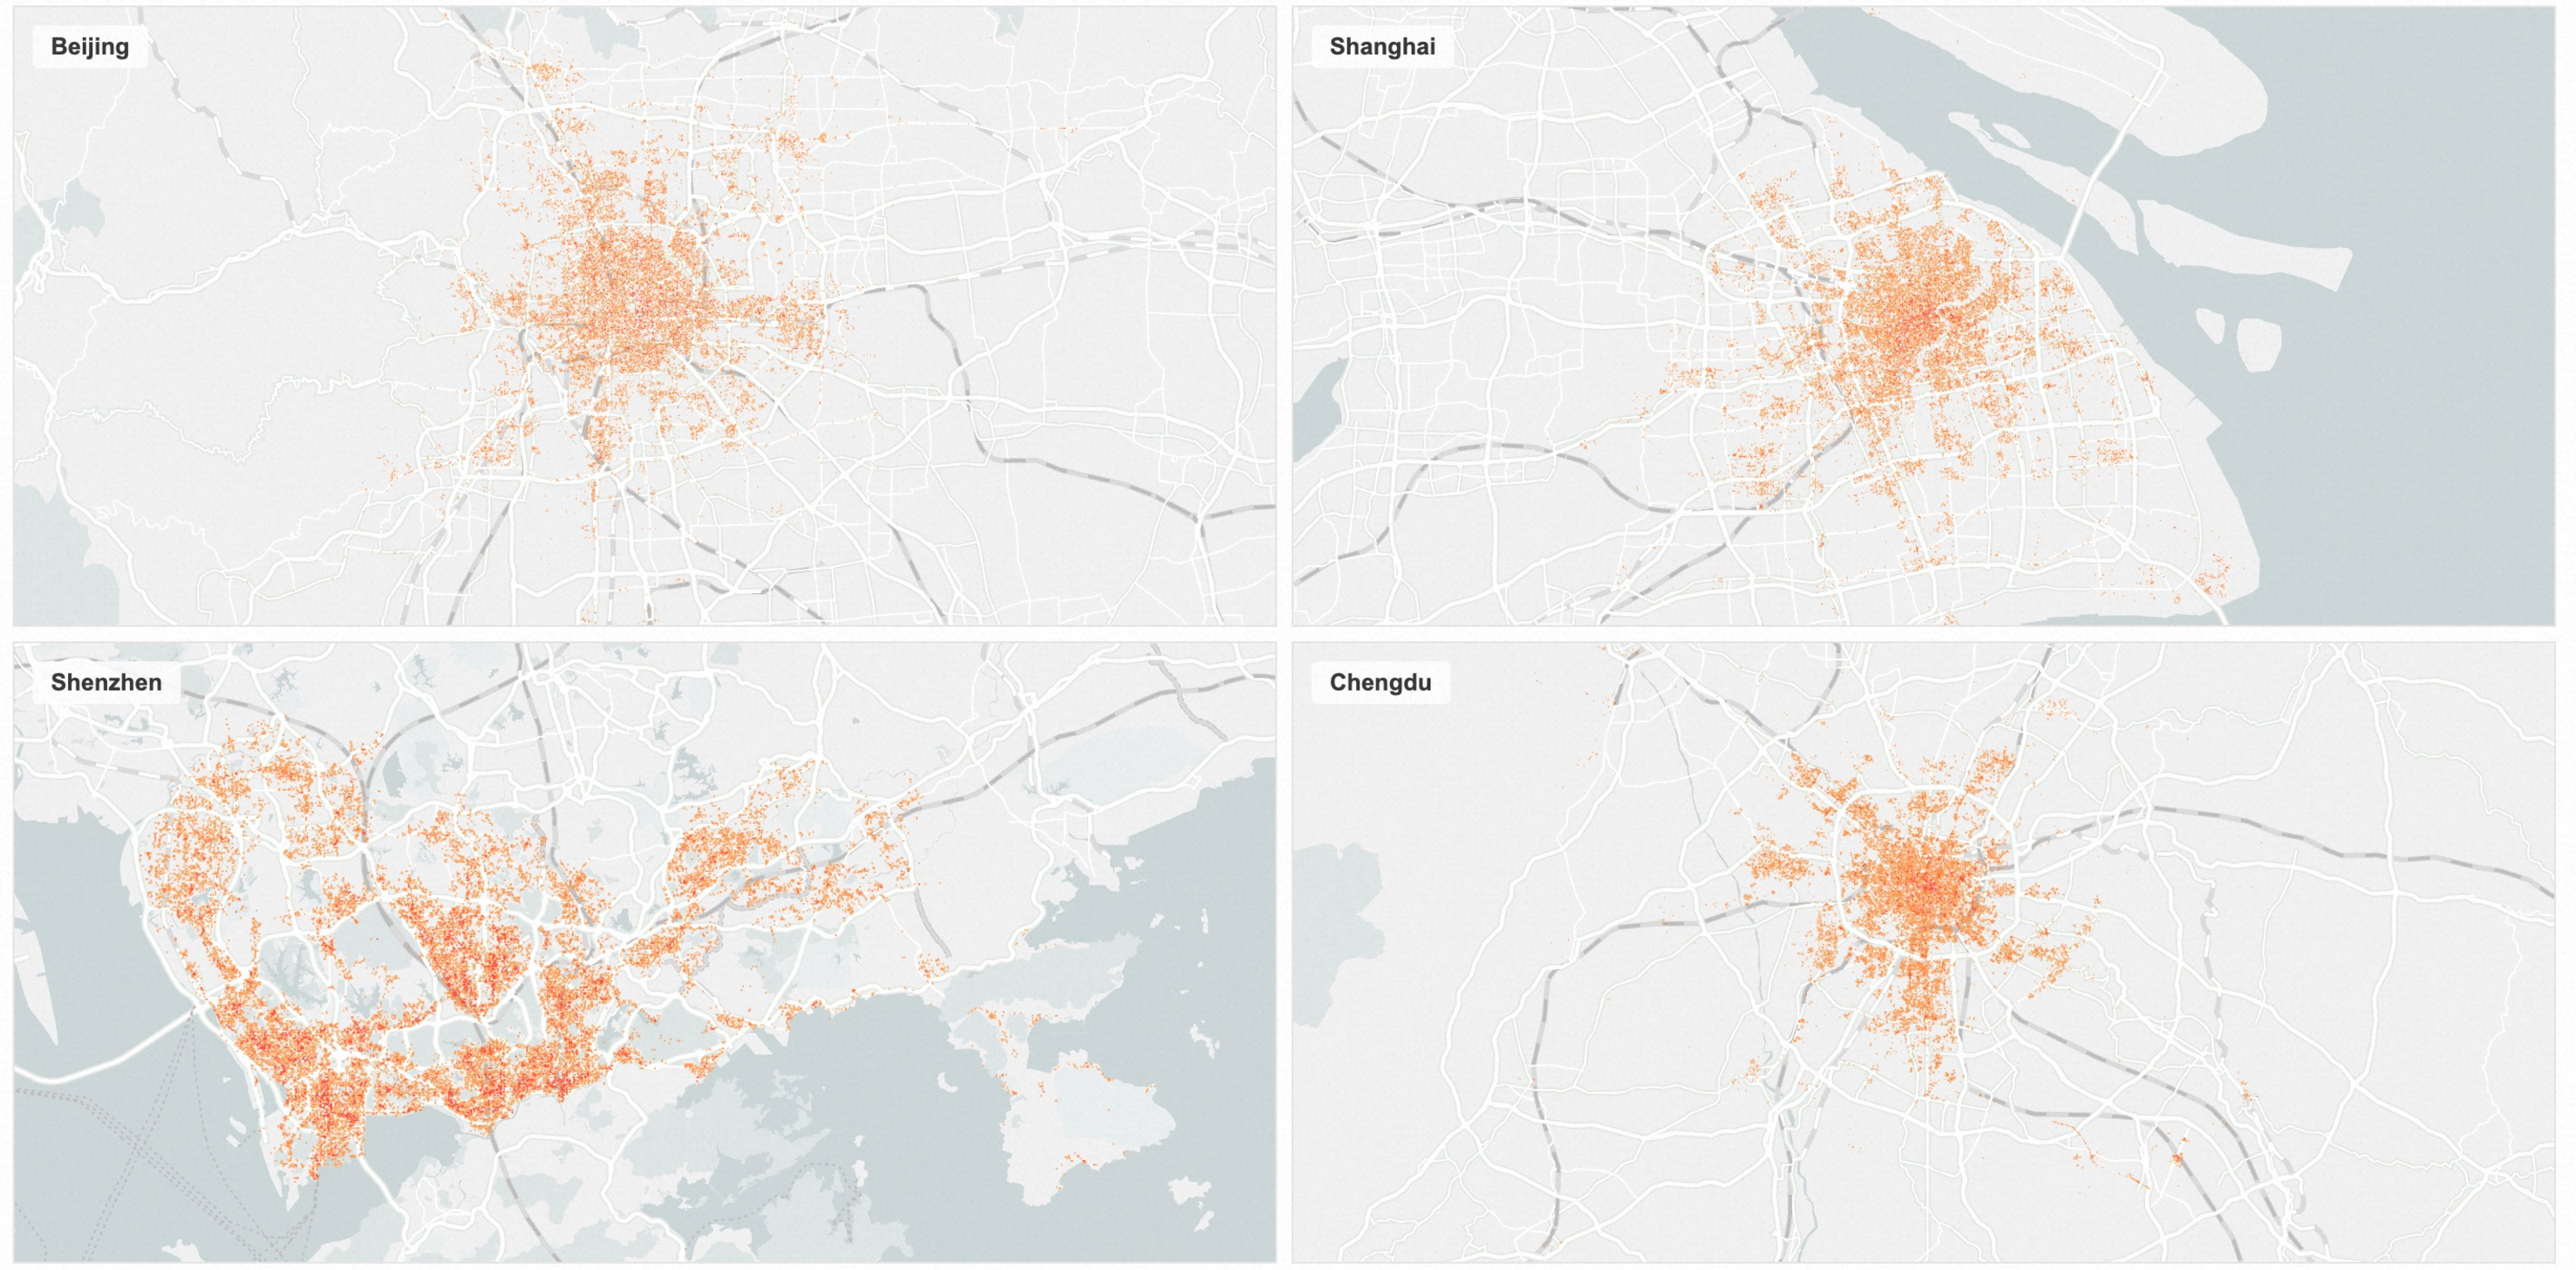
\includegraphics[width=\textwidth]{figures/heatmap_4cities.pdf}
\caption{Geographic distribution of route planning origins across the four cities. Density reflects real-world transit demand concentration in urban cores.}
\label{fig:heatmap}
\end{figure}

\section{CPT Corpus Sample}
\label{app:cpt_sample}

The CPT corpus consists of two complementary components: (1)~\textbf{session records} derived from real-world transit planning sessions, each pairing an origin--destination request with candidate routes, and (2)~\textbf{static descriptions} of transit lines and stations. The original corpus is in Chinese; English translations are provided below for readability.

\paragraph{Session Records.}
Each session record follows a \textit{query~$\rightarrow$~route options} structure. The query specifies the city, origin--destination GPS coordinates, and POI names. Each candidate route details the transport mode, line name, per-segment distance and time, fare, boarding/alighting stations with coordinates, and the complete station ID sequence.

\begin{tcolorbox}[colback=gray!3, colframe=black!40, boxrule=0.4pt, arc=2pt, left=6pt, right=6pt, top=4pt, bottom=4pt, fontupper=\small, fontlower=\small, breakable, title={\small\textbf{CPT Session Record}}]
\textbf{Query:} How to get to Yongtai Dongli? \\
\textbf{City:} Beijing \quad \textbf{Origin:} 116.398261, 39.889556 \quad \textbf{Dest:} 116.358844, 40.034880

\tcblower

\textbf{Option 1} \textit{(Subway, 21.3\,km, 55\,min, 5\,yuan)} \\[2pt]
Walk 170\,m (2\,min) to bus-899931 (Zhushikou, 116.398375, 39.889961). \\
Take Subway Line 8 to bus-893448 (Yongtaizhuang, 116.354580, 40.037728), 20.3\,km, 41\,min. \\
Walk 880\,m to destination. \\[2pt]
\textit{Stations:} bus-899931, bus-900093, \ldots, bus-893448.

\vspace{4pt}
\noindent\dashrule
\vspace{4pt}

\textbf{Option 2} \textit{(Bus, 20.8\,km, 1h\,55min, 5\,yuan)} \\[2pt]
Walk 524\,m to bus-899401 (Banzhang Rd, 116.394073, 39.890199). \\
Take Bus 5 to bus-897760 (Madian Bridge S., 116.397834, 39.959271), 10.7\,km, 54\,min. \\
\textit{[Transfer]} Take Bus 625 to bus-892356 (Qinghe, 116.348232, 40.030627), 8.3\,km, 34\,min. \\
Walk 1.4\,km to destination. \\[2pt]
\textit{Stations:} bus-899401, \ldots, bus-897760, [transfer], bus-897760, \ldots, bus-892356.
\end{tcolorbox}

\paragraph{Static Descriptions.}
The corpus also includes structured descriptions of individual transit lines and stations, encoding attributes such as route length, stop count, operating hours, fare policy, coordinates, and connectivity to neighboring stations.

\begin{tcolorbox}[colback=gray!3, colframe=black!40, boxrule=0.4pt, arc=2pt, left=6pt, right=6pt, top=4pt, bottom=4pt, fontupper=\small, fontlower=\small, breakable, title={\small\textbf{CPT Static Descriptions}}]
\textbf{Line Description} \\[2pt]
\textit{Line:} Zhuan-117 (Tiantongyuan North Hub -- Yandan) \\
\textit{Type:} Micro-circulation bus \quad \textit{Length:} 5.3\,km \quad \textit{Stops:} 9 \\
\textit{Hours:} 05:50--22:30 \quad \textit{Fare:} 2\,yuan (flat) \\[2pt]
\textit{Stop sequence:} \\
\#1 Tiantongyuan North Hub (bus-901618) $\rightarrow$
\#2 Tiantong Beiyuan Block\,1 North Gate (bus-902625) $\rightarrow$
\#3 Tiantong Beiyuan Block\,2 North Gate (bus-903364) $\rightarrow$
\#4 Shiziying (bus-904346) $\rightarrow$
\#5 Tiantong Beiyuan Block\,3 North Gate (bus-904981) $\rightarrow$
\#6 Qixing Rd South (bus-905417) $\rightarrow$
\#7 Yanchengyuan Intersection South (bus-905008) $\rightarrow$
\#8 Yanchengyuan (bus-905518) $\rightarrow$
\#9 Yandan (bus-905652).

\tcblower

\textbf{Station Description} \\[2pt]
\textit{Station:} Pinggu No.4 Middle School (bus-1000071) \\
\textit{District:} Pinggu, Beijing \quad \textit{Lines served:} 2 \\
\textit{Coordinates:} (117.089436, 40.130547) \\[2pt]
\textit{Connectivity:} From this station, take Line Ping-2 (Passenger Terminal -- Pinggu No.7 Primary School) to Yuming School (bus-1000202).
\end{tcolorbox}

\section{Benchmark SFT Examples}
\label{app:benchmark_examples}

Each benchmark task uses a standardized prompt--label format. The prompt contains a system instruction describing the task, followed by a user request with origin--destination coordinates. The label is a structured JSON object encoding the expected route. Below we show representative examples for all three tasks; the original text is in Chinese and translated here for readability.

\paragraph{Optimal Route Generation.}
Given origin--destination coordinates, the model generates a single optimal transit route as a structured JSON object.
\begin{tcolorbox}[colback=gray!3, colframe=black!40, boxrule=0.4pt, arc=2pt, left=6pt, right=6pt, top=4pt, bottom=4pt, fontupper=\small, fontlower=\small, breakable, title={\small\textbf{Prompt \& Label}}]
\textbf{System Prompt} \\[2pt]
You are a public transit route planning expert, familiar with bus and subway networks.

\textit{Task:} \textbf{Given the user's origin and destination coordinates, plan an optimal transit route.}

\textit{Input:} \texttt{query}, \texttt{start} (lng, lat), \texttt{end} (lng, lat), \texttt{city}.

\textit{Output (JSON):} \texttt{line\_sequence}, \texttt{station\_sequence} (with \texttt{[Transfer]}), \texttt{total\_distance}, \texttt{total\_time}, \texttt{total\_fare}, \texttt{start\_transfer\_mode/distance}, \texttt{end\_transfer\_mode/distance}.

\tcblower

\textbf{Prompt} \\[2pt]
\texttt{\{"query": "How to get to BIT (South Gate)?", "start": "116.395310,39.963284",} \\
\texttt{~"end": "116.316356,39.957053", "city": "Beijing"\}}

\vspace{6pt}
\textbf{Label} \\[2pt]
\texttt{\{"line\_sequence": ["Subway Line 12", "Subway Line 4"],} \\
\texttt{~"station\_sequence": ["bus-899733", "bus-898054", ..., "bus-888019",} \\
\texttt{~~"[Transfer]", "bus-887631", "bus-887990"],} \\
\texttt{~"total\_distance": "9.2 km", "total\_time": "49 min", "total\_fare": "4 yuan",} \\
\texttt{~"start\_transfer\_mode": "walking", "start\_transfer\_distance": "896 m",} \\
\texttt{~"end\_transfer\_mode": "walking", "end\_transfer\_distance": "759 m"\}}
\end{tcolorbox}

\paragraph{Preference-Aware Planning.}
In addition to coordinates, the prompt includes a user preference constraint. The model must produce a route that satisfies the stated preference while maintaining overall quality.
\begin{tcolorbox}[colback=gray!3, colframe=black!40, boxrule=0.4pt, arc=2pt, left=6pt, right=6pt, top=4pt, bottom=4pt, fontupper=\small, fontlower=\small, breakable, title={\small\textbf{Prompt \& Label}}]
\textbf{System Prompt} \\[2pt]
You are a public transit route planning expert, familiar with bus and subway networks.

\textit{Task:} \textbf{Given the user's origin and destination coordinates along with a stated preference, plan a transit route that satisfies the preference while maintaining overall route quality.}

\textit{Input:} \texttt{query} (with preference), \texttt{start} (lng, lat), \texttt{end} (lng, lat), \texttt{city}.

\textit{Output (JSON):} \texttt{line\_sequence}, \texttt{station\_sequence} (with \texttt{[Transfer]}), \texttt{total\_distance}, \texttt{total\_time}, \texttt{total\_fare}, \texttt{start\_transfer\_mode/distance}, \texttt{end\_transfer\_mode/distance}.

\tcblower

\textbf{Prompt} \\[2pt]
\texttt{\{"query": "How to get to Jingshan Park by bus? Bus-first.",} \\
\texttt{~"start": "116.421180,39.880405", "end": "116.396551,39.925875", "city": "Beijing"\}}

\vspace{6pt}
\textbf{Label} \\[2pt]
\texttt{\{"line\_sequence": ["Bus 128 (Xiaocunqiao N.--Beijing No.39 Middle School)"],} \\
\texttt{~"station\_sequence": ["bus-903008", "bus-902952", "bus-902743", "bus-902705",} \\
\texttt{~~"bus-902688", "bus-902629", "bus-902600", "bus-902571", "bus-902555",} \\
\texttt{~~"bus-902495", "bus-902472", "bus-901722", "bus-900713", "bus-899614"],} \\
\texttt{~"total\_distance": "7.0 km", "total\_time": "53 min", "total\_fare": "2 yuan",} \\
\texttt{~"start\_transfer\_mode": "walking", "start\_transfer\_distance": "143 m",} \\
\texttt{~"end\_transfer\_mode": "walking", "end\_transfer\_distance": "145 m"\}}
\end{tcolorbox}

\paragraph{Multi-Route Generation.}
The model produces three diverse transit routes for a single origin--destination pair. Each route should adopt a different mode or line combination to offer meaningful travel alternatives, while maintaining overall route quality.
\begin{tcolorbox}[colback=gray!3, colframe=black!40, boxrule=0.4pt, arc=2pt, left=6pt, right=6pt, top=4pt, bottom=4pt, fontupper=\small, fontlower=\small, breakable, title={\small\textbf{Prompt \& Label}}]
\textbf{System Prompt} \\[2pt]
You are a public transit route planning expert, familiar with bus and subway networks.

\textit{Task:} \textbf{Given origin--destination coordinates and city, plan three diverse transit routes using different mode or line combinations.}

\textit{Input:} \texttt{query}, \texttt{start} (lng, lat), \texttt{end} (lng, lat), \texttt{city}.

\textit{Output (JSON):} Three route objects (\texttt{first}, \texttt{second}, \texttt{third}), each containing \texttt{route\_tag}, \texttt{line\_sequence}, \texttt{station\_sequence}, \texttt{total\_distance}, \texttt{total\_time}, \texttt{total\_fare}, \texttt{start/end\_transfer\_mode/distance}.

\tcblower

\textbf{Prompt} \\[2pt]
\texttt{\{"query": "How to get from Tongji Univ.\ to Shanghai Pudong Intl.\ Airport} \\
\texttt{~by public transit? Give me a few options.",} \\
\texttt{~"start": "121.513244,31.282003", "end": "121.808681,31.142267",} \\
\texttt{~"city": "Shanghai"\}}

\vspace{6pt}
\textbf{Label} \\[4pt]
\texttt{\{"first": \{"route\_tag": "Subway",} \\
\texttt{~~"line\_sequence": ["Subway Line 18", "Subway Line 2"],} \\
\texttt{~~"station\_sequence": ["bus-1670095", \ldots, "bus-1677113",} \\
\texttt{~~~"[Transfer]", "bus-1677227", \ldots, "bus-1701975"],} \\
\texttt{~~"total\_distance": "41.1 km", "total\_time": "1h 22min", "total\_fare": "7 yuan",} \\
\texttt{~~"start\_transfer\_mode": "walking", "start\_transfer\_distance": "169 m",} \\
\texttt{~~"end\_transfer\_mode": "walking", "end\_transfer\_distance": "22 m"\},} \\[3pt]
\texttt{~"second": \{"route\_tag": "Bus+Subway",} \\
\texttt{~~"line\_sequence": ["Subway Line 18", "Maglev Line"],} \\
\texttt{~~"station\_sequence": [\ldots], \ldots\},} \\[3pt]
\texttt{~"third": \{"route\_tag": "Bus",} \\
\texttt{~~"line\_sequence": ["Airport Express Line 4"],} \\
\texttt{~~"station\_sequence": [\ldots], \ldots\}\}}
\end{tcolorbox}

\section{Evaluation Metrics}
\label{app:metrics}

This appendix provides the formal definitions of all evaluation metrics introduced in Section~\ref{benchmark}. The metrics cover four complementary dimensions: \textit{Connectivity} verifies structural correctness of the predicted station sequence; \textit{Access Feasibility} checks whether first/last-mile access is physically plausible; \textit{Route Overlap} measures structural match between predicted and label routes; and \textit{Numeric Field Accuracy} assesses the accuracy of predicted numeric fields. In addition, Preference-Aware Planning and Multi-Route Generation define task-specific metrics for preference compliance and route diversity, respectively. Table~\ref{tab:metric_abbr} provides a quick-reference summary of all metric abbreviations.

\begin{table}[h]
\centering
\small
\caption{Evaluation metrics and abbreviations.}
\label{tab:metric_abbr}
\renewcommand{\arraystretch}{1.05}
\resizebox{\textwidth}{!}{
\begin{tabular}{@{}ll p{0.52\textwidth}@{}}
\toprule
\textbf{Metric} & \textbf{Abbr.} & \textbf{Description} \\
\midrule
\multicolumn{3}{l}{\textit{Evaluation Dimensions}} \\[2pt]
Connectivity & Conn & Consecutive stations reachable in the transit network \\
\cdashline{1-3}[0.4pt/3pt]
Access Feasibility & & First/last-mile access plausibility \\
\quad Station Grounding & SG & First/last station within mode-specific distance of OD \\
\quad Distance Plausibility & DP & Pred.\ access dist.\ matches OD-to-station straight-line \\
\cdashline{1-3}[0.4pt/3pt]
Route Overlap & & Structural match between predicted and label routes \\
\quad Line Overlap & LO & IoU of full line sets including access segments \\
\quad Station Sequence Overlap & SSO & IoU of station ID sets \\
\quad Route Exact Match & REM & Fraction of samples with LO\,=\,1 and SSO\,=\,1 \\
\cdashline{1-3}[0.4pt/3pt]
Numeric Field Accuracy & & Accuracy of predicted numeric fields \\
\quad Estimation Accuracy & EA & Avg.\ pass rate over distance, time, and fare \\
\quad Mean Absolute Percentage Error & MAPE & Avg.\ relative error over distance, time, and fare \\
\midrule
\multicolumn{3}{l}{\textit{Task-specific Metrics}} \\[2pt]
Preference Compliance & PC & Stated preference satisfied \\
Route Diversity & RD & Pairwise line-set dissimilarity \\
\bottomrule
\end{tabular}
}
\end{table}

\subsection{Connectivity}

Connectivity is the first evaluation dimension, verifying that the predicted station sequence forms a structurally valid path in the transit network. A predicted route is \emph{connected} if and only if every consecutive station pair $(s_i, s_{i+1})$ in the generated sequence is reachable, either on the same line or via a valid transfer recorded in the city's transfer table. Connectivity is reported as the percentage of test samples whose predicted routes are fully connected:
\begin{equation}
\text{Conn} = \frac{1}{N}\sum_{i=1}^{N} \mathbf{1}\!\left[\,\forall\, 1 \leq j < L^{(i)},\; (s_j^{(i)}, s_{j+1}^{(i)}) \in \mathcal{E}\,\right]
\end{equation}
where $L^{(i)}$ is the length of the predicted station sequence for sample $i$ and $\mathcal{E}$ is the set of station pairs that are adjacent on a shared line or connected via an inter-line transfer. Connectivity serves as a prerequisite: all subsequent metrics except task-specific ones (PC, RD) are computed only on connected samples.

\subsection{Access Feasibility}

Access Feasibility is the second evaluation dimension. While Connectivity verifies reachability among intermediate stations, this metric validates the first/last-mile segments, jointly ensuring that the entire origin-to-destination path is both connected and accessible. For each access segment, let $d_{\text{geo}}$ denote the straight-line (Haversine) distance between the origin/destination and the predicted boarding/alighting station, and let $d_{\text{pred}}$ denote the predicted access distance. Let $a_{\mathrm{s}}^{(i)}$ and $a_{\mathrm{e}}^{(i)}$ denote the start and end access segments of sample $i$.

\paragraph{Station Grounding.} This metric evaluates whether the model can implicitly map raw GPS coordinates to nearby transit stations without any explicit coordinate-to-station lookup module. A high pass rate indicates that the model has learned spatial grounding purely from training data. The straight-line distance between the origin/destination and the predicted boarding/alighting station must not exceed a mode-specific threshold:
\begin{center}
\small
\begin{tabular}{l@{\hspace{2em}}c}
\toprule
Access Mode & Threshold $\tau_m$ \\
\midrule
Walking & 3\,km \\
Cycling & 5\,km \\
Taxi & 10\,km \\
\bottomrule
\end{tabular}
\end{center}
\noindent The pass rate is:
\begin{equation}
\text{SG} = \frac{1}{N}\sum_{i=1}^{N} \mathbf{1}\!\left[\,d_{\text{geo}}(a_{\mathrm{s}}^{(i)}) \leq \tau_{m_{\mathrm{s}}} \;\wedge\; d_{\text{geo}}(a_{\mathrm{e}}^{(i)}) \leq \tau_{m_{\mathrm{e}}}\,\right]
\end{equation}
where $\tau_{m}$ is the mode-specific threshold from the table above.

\paragraph{Distance Plausibility.} While Station Grounding validates spatial proximity, this metric further verifies that the predicted access distance is physically realistic rather than a hallucinated value. A plausible access distance must satisfy two conditions:
\begin{itemize}[leftmargin=2em, itemsep=2pt]
\item $d_{\text{pred}} \geq d_{\text{geo}}$ \quad (predicted distance must not fall below the geometric lower bound)
\item $d_{\text{pred}} \leq 3 \cdot d_{\text{geo}}$ \quad (predicted distance not unreasonably large)
\end{itemize}
\noindent Let $\phi(a) = \mathbf{1}[d_{\text{geo}}(a) \leq d_{\text{pred}}(a) \leq 3 \cdot d_{\text{geo}}(a)]$. The pass rate is:
\begin{equation}
\text{DP} = \frac{1}{N}\sum_{i=1}^{N} \phi(a_{\mathrm{s}}^{(i)}) \cdot \phi(a_{\mathrm{e}}^{(i)})
\end{equation}
The upper-bound factor of 3 is empirically set as a plausibility threshold: real-world access distances rarely exceed three times the straight-line distance, so predictions beyond this bound are considered implausible.

\subsection{Route Overlap}
Route Overlap is the third evaluation dimension, quantifying the structural match between a predicted route and its ground-truth counterpart. For Optimal Route Generation and Preference-Aware Planning, the single predicted route is directly compared against the label. For Multi-Route Generation, the first predicted route is used for comparison, as the task requires the first output route to be the ground-truth route, and the training and evaluation data are constructed accordingly. Both Line Overlap and Station Sequence Overlap are defined via Intersection-over-Union (IoU):
\begin{equation}
\text{IoU}(A, B) = \frac{|A \cap B|}{|A \cup B|}
\end{equation}
For \textit{Line Overlap} ($\text{LO}$), $A$ and $B$ are the full line sets of the predicted and ground-truth routes, including first/last-mile access segments (e.g., cycling, taxi). For \textit{Station Sequence Overlap} ($\text{SSO}$), $A$ and $B$ are the corresponding station ID sets.

\textit{Route Exact Match} ($\text{REM}$) measures the fraction of samples whose predicted and ground-truth routes are structurally identical in both lines and stations:
\begin{equation}
\text{REM} = \frac{1}{N}\sum_{i=1}^{N} \mathbf{1}\!\left[\,\text{LO}^{(i)} = 1 \;\wedge\; \text{SSO}^{(i)} = 1\,\right]
\end{equation}

\subsection{Numeric Field Accuracy}

Numeric Field Accuracy is the fourth evaluation dimension, measuring how accurately the model predicts route-level numeric attributes. Let $\mathcal{F} = \{\text{distance}, \text{time}, \text{fare}\}$ denote the set of route-level numeric fields. Evaluation is restricted to samples that achieve Route Exact Match, i.e., both $\text{LO} = 1$ and $\text{SSO} = 1$, as only under this condition do the ground-truth numeric fields constitute valid references. Let $\mathcal{M}$ denote this set of matched samples.

\textbf{\textit{Estimation Accuracy (EA).}}
For each field $f \in \mathcal{F}$, a prediction passes if it satisfies \textit{either} a relative tolerance \textit{or} an absolute tolerance:
\begin{equation}
\text{EA}_f = \frac{1}{|\mathcal{M}|}\sum_{i \in \mathcal{M}} \mathbf{1}\!\left[\frac{|\hat{y}_f^{(i)} - y_f^{(i)}|}{y_f^{(i)}} \leq 10\% \;\;\text{or}\;\; |\hat{y}_f^{(i)} - y_f^{(i)}| \leq \epsilon_f\right]
\end{equation}
where $\epsilon_{\text{time}} = 5\,\text{min}$, $\epsilon_{\text{distance}} = 500\,\text{m}$, and $\epsilon_{\text{fare}} = 1\,\text{CNY}$. The reported EA is the average across all fields: $\text{EA} = \frac{1}{|\mathcal{F}|}\sum_{f \in \mathcal{F}} \text{EA}_f$. The dual-tolerance design ensures that predictions with small absolute error but inflated relative error (due to small denominators) are not penalized, and likewise for predictions with small relative error but large absolute difference.

\textbf{\textit{Mean Absolute Percentage Error (MAPE).}} While EA provides a binary pass/fail judgment, MAPE quantifies the continuous error magnitude. The per-field MAPE is:
\begin{equation}
\text{MAPE}_f = \frac{1}{|\mathcal{M}|}\sum_{i \in \mathcal{M}} \frac{|\hat{y}_f^{(i)} - y_f^{(i)}|}{y_f^{(i)}}
\end{equation}
The reported MAPE is the average across all fields: $\text{MAPE} = \frac{1}{|\mathcal{F}|}\sum_{f \in \mathcal{F}} \text{MAPE}_f$.

\subsection{Preference Compliance}

Preference Compliance is a task-specific metric for Preference-Aware Planning that evaluates whether the model can generate routes adhering to an explicit user preference. Let $r_{\text{gt}}$ denote the ground-truth route. For each preference type, compliance is determined by a hard rule:

\begin{center}
\small
\begin{tabular}{lp{8cm}}
\toprule
\textbf{Preference} & \textbf{Compliance Rule} \\
\midrule
Subway-first & The predicted route contains at least one subway segment. \\
Bus-first & The predicted route contains at least one bus segment. \\
Fewer transfers & $N_{\text{transfers}}^{\text{pred}} \leq N_{\text{transfers}}^{\text{gt}}$ \\
Shortest time & $T^{\text{pred}} \leq \alpha \cdot T^{\text{gt}}$, where $\alpha = 1.1$ \\
\bottomrule
\end{tabular}
\end{center}

\noindent The tolerance factor $\alpha$ for shortest time accounts for the inherent imprecision of predicted numeric values. Preference Compliance is reported as the percentage of test samples whose predicted routes satisfy the corresponding rule. Note that the theoretical upper bound of this metric is below 100\%: routes that strictly satisfy a preference may have poor overall quality, so the ground-truth labels prioritize route quality and do not always comply with the hard rule.

\subsection{Route Diversity}

Route Diversity is a task-specific metric for Multi-Route Generation that evaluates whether the model can produce structurally distinct alternatives rather than near-duplicate routes. For each sample, the pairwise dissimilarity over all $\binom{3}{2} = 3$ route pairs is:
\begin{equation}
\text{RD}^{(k)} = \frac{1}{3}\sum_{(i,j)}(1 - \text{IoU}(\mathcal{L}_i^{(k)}, \mathcal{L}_j^{(k)}))
\end{equation}
where $\mathcal{L}_i^{(k)}$ is the full line set of route $i$ in sample $k$, including cycling and taxi access segments. The reported metric is the average over all $N$ test samples: $\text{RD} = \frac{1}{N}\sum_{k=1}^{N}\text{RD}^{(k)}$. Values range from 0 (all routes identical) to 1 (no shared lines). Route Diversity should be evaluated jointly with the four evaluation dimensions, as maximizing diversity alone may sacrifice route quality. The two metrics together capture whether the model produces varied yet practically viable alternatives.

\section{Hyperparameters}
\label{app:hyperparams}

Table~\ref{tab:hyperparams} summarizes all hyperparameters used in training and inference. During CPT, all sequences are packed to the fixed sequence length with no padding, so the training budget is measured in steps rather than epochs. During SFT, sequences are not packed and instead processed at their natural length with standard padding; the loss is computed only on the response tokens, with prompt tokens masked. Both stages use DeepSpeed ZeRO-3 \cite{rajbhandari2020zero} for distributed training. Greedy decoding with a fixed seed is used for all benchmark evaluations to ensure deterministic and reproducible outputs.

\begin{table}[t]
\centering
\caption{Hyperparameters for training and inference.}
\label{tab:hyperparams}
\small
\setlength{\tabcolsep}{8pt}
\begin{tabular}{@{}lcc@{}}
\toprule
\textbf{Hyperparameter} & \textbf{CPT} & \textbf{SFT} \\
\midrule
\multicolumn{3}{l}{\textit{Model}} \\[2pt]
\quad Backbone & \multicolumn{2}{c}{Qwen3-Base (0.6B / 1.7B / 4B)} \\
\quad Initialization & Base weights & CPT checkpoint \\
\quad Added tokens & \multicolumn{2}{c}{120,845 station IDs} \\
\midrule
\multicolumn{3}{l}{\textit{Optimization}} \\[2pt]
\quad Learning rate & 2e-5 & 2e-5 \\
\quad LR scheduler & Cosine & Cosine \\
\quad Optimizer & AdamW & AdamW \\
\quad Warmup steps & 500 & 15 \\
\quad Weight decay & 0.01 & 0.01 \\
\quad Precision & bf16 & bf16 \\
\quad Distributed strategy & \multicolumn{2}{c}{DeepSpeed ZeRO-3} \\
\quad Loss masking & Full sequence & Response only \\
\midrule
\multicolumn{3}{l}{\textit{Data \& Compute}} \\[2pt]
\quad Sequence length & 4,096 (packed) & Dynamic \\
\quad Per-device batch size & 4 & 8 \\
\quad Gradient accumulation & 4 & 4 \\
\quad Number of devices & 64 PPUs (96\,GB) & 8 PPUs (96\,GB) \\
\quad Effective batch size & 1,024 & 256 \\
\quad Training budget & 15,000 steps & 1 epoch \\
\midrule
\multicolumn{3}{l}{\textit{Inference}} \\[2pt]
\quad Decoding strategy & \multicolumn{2}{c}{Greedy} \\
\quad Max new tokens & \multicolumn{2}{c}{4,096} \\
\quad Input cutoff length & \multicolumn{2}{c}{2,048} \\
\quad Seed & \multicolumn{2}{c}{1} \\
\bottomrule
\end{tabular}
\end{table}

\section{Additional Experiments}
\label{app:additional_exp}

\subsection{CPT Training Dynamics}
\label{app:cpt_loss}

Figure~\ref{fig:cpt_loss} plots the CPT training loss for the three backbone models over approximately 15k steps ($\approx$\,3 epochs). All models drop from $>$\,1.0 to approximately 0.1 within the first 2k steps, indicating that domain-specific token distributions are learned early regardless of model capacity. The inset (steps 4k--14k) reveals a stable ordering Qwen3-4B $<$ Qwen3-1.7B $<$ Qwen3-0.6B in loss, consistent with downstream performance in Tables~\ref{tab:task1_results}--\ref{tab:task3_results}. Loss continues to decrease through Epochs~2 and~3 (e.g., 4B: 0.084\,$\to$\,0.070), suggesting that later epochs further consolidate transit-domain knowledge rather than overfit. Wall-clock training time on 64 PPUs is approximately 6 days for Qwen3-4B, 3 days for Qwen3-1.7B, and 1.5 days for Qwen3-0.6B, scaling approximately with model size.

\begin{figure}[t]
\centering
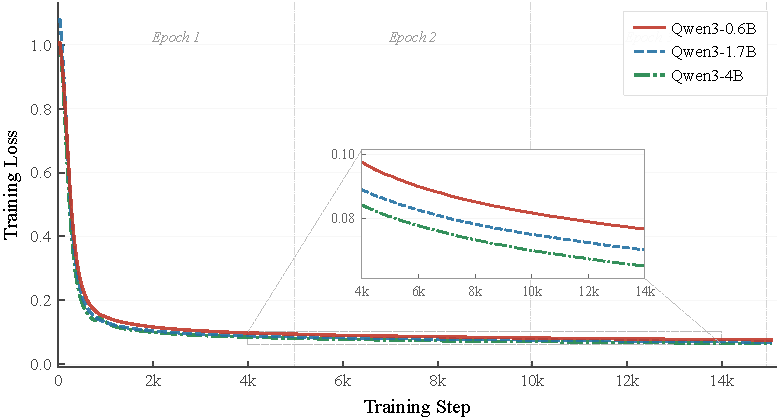
\includegraphics[width=0.85\textwidth]{figures/cpt_loss_comparison.pdf}
\caption{CPT training loss curves for Qwen3-0.6B, Qwen3-1.7B, and Qwen3-4B over $\approx$\,15k steps. The inset magnifies steps 4k--14k to highlight the sustained loss reduction and the capacity gap across model sizes.}
\label{fig:cpt_loss}
\end{figure}

\subsection{Single-City vs.\ Multi-City CPT}
\label{app:single_city}

Our framework introduces every station ID as a new token in the vocabulary. Scaling from one city to four increases the station vocabulary from 38{,}792 to 120{,}845, a 3.1$\times$ expansion. Because the total CPT data volume is held constant, each Beijing station receives roughly one-third as many training examples under the multi-city setting. This ablation examines whether the resulting token-level sparsity degrades per-city performance, and whether cross-city training provides compensating knowledge transfer. To this end, we train a single-city model on Beijing data only, using the same Qwen3-4B base and identical CPT data volume as the four-city model. Both models are evaluated on the Beijing test set of 10{,}000 samples for Optimal Route Generation. Table~\ref{tab:single_city} reports the comparison.

\begin{table}[t]
\centering
\caption{Single-city vs.\ multi-city CPT on \textbf{Optimal Route Generation}, evaluated on the Beijing test set with 10{,}000 samples. The single-city model is trained on Beijing data only, while the multi-city model covers all four cities. Both use the same total CPT data volume and identical SFT data. $\Delta$ denotes the change from Beijing-only to four-city. $\uparrow$\,/\,$\downarrow$ indicate higher/lower is better. \textbf{Bold}: better of the two.}
\label{tab:single_city}
\small
\setlength{\tabcolsep}{6pt}
\renewcommand{\arraystretch}{1.05}
\scalebox{1.05}{
\begin{tabular}{@{}l@{\enspace}c ccc@{}}
\toprule
\textbf{Metric} & & \textbf{Beijing-Only} & \textbf{Four-City} & \textbf{$\Delta$} \\
\midrule
Connectivity & $\uparrow$ & \textbf{95.8\%} & 95.5\% & $-$0.3 \\
\cdashline{1-5}[0.4pt/3pt]
Station Grounding & $\uparrow$ & 97.5\% & \textbf{97.8\%} & \textcolor{ForestGreen}{+0.3} \\
Distance Plausibility & $\uparrow$ & \textbf{89.7\%} & 88.8\% & $-$0.9 \\
\cdashline{1-5}[0.4pt/3pt]
Line Overlap & $\uparrow$ & \textbf{0.853} & 0.845 & $-$0.008 \\
Station Sequence Overlap & $\uparrow$ & \textbf{0.853} & 0.839 & $-$0.014 \\
Route Exact Match & $\uparrow$ & \textbf{74.0\%} & 70.5\% & $-$3.5 \\
\cdashline{1-5}[0.4pt/3pt]
Estimation Accuracy & $\uparrow$ & 97.1\% & \textbf{97.6\%} & \textcolor{ForestGreen}{+0.5} \\
MAPE & $\downarrow$ & \textbf{1.30\%} & 1.63\% & +0.33 \\
\bottomrule
\end{tabular}
}
\end{table}

Despite a 3.1$\times$ vocabulary expansion and proportionally fewer per-station training examples, the four-city model trails the Beijing-only model by only 3.5 percentage points in Route Exact Match. This confirms that token-level sparsity introduced by city scaling does not cause significant performance degradation. Station Grounding and Estimation Accuracy are slightly higher under multi-city training, suggesting that shared spatial patterns across cities provide positive knowledge transfer that partially compensates for reduced per-station coverage. The minor increase in MAPE and decrease in route-level overlap metrics represent a modest cost of distributing the same data budget across a larger station vocabulary. These results validate that the proposed framework scales gracefully to additional cities, directly supporting the future direction of extending coverage to broader geographies.

\subsection{Effect of Continual Pre-Training}
\label{app:cpt_ablation}

To isolate the contribution of continual pre-training, we construct an SFT-only baseline that bypasses the CPT stage and instead trains the base Qwen3-4B model directly on the same volume of session data used by CPT-25\%, reformatted as supervised fine-tuning examples. This ensures that the comparison controls for total data volume rather than merely removing a training stage. We additionally include CPT-25\%, CPT-100\%, and the multi-task 4B-Joint model. All variants share identical station token vocabulary and are evaluated on the same test set. Each configuration is evaluated under both standard text input and GPS-only input to probe the robustness of the learned representations. Table~\ref{tab:cpt_ablation} reports the results.

\begin{table}[t]
\centering
\caption{Effect of continual pre-training on \textbf{Optimal Route Generation} with 10{,}000 test samples. SFT-only bypasses the CPT stage and trains on the same session data volume as CPT-25\%, reformatted as SFT examples. All variants share identical station token vocabulary and test set. Each configuration is evaluated under standard text and GPS-only input. $\uparrow$\,/\,$\downarrow$ indicate higher/lower is better. \textbf{Bold}: best; \underline{underline}: second best.}
\label{tab:cpt_ablation}
\small
\setlength{\tabcolsep}{3pt}
\renewcommand{\arraystretch}{1.05}
\scalebox{1.0}{
\begin{tabular}{@{}l@{\enspace}c cccc@{}}
\toprule
\textbf{Metric} & & \textbf{SFT-only} & \textbf{CPT-25\%} & \textbf{CPT-100\%} & \textbf{4B-Joint} \\
\midrule
\multicolumn{6}{@{}l}{\textit{Standard input}} \\
Connectivity & $\uparrow$ & \underline{97.3\%} & 95.9\% & 97.0\% & \textbf{97.9\%} \\
Station Grounding & $\uparrow$ & 97.2\% & 97.7\% & \underline{98.5\%} & \textbf{98.9\%} \\
Distance Plausibility & $\uparrow$ & 90.7\% & 87.4\% & \underline{91.0\%} & \textbf{92.9\%} \\
Line Overlap & $\uparrow$ & 0.820 & 0.811 & \underline{0.828} & \textbf{0.835} \\
Station Sequence Overlap & $\uparrow$ & 0.835 & 0.816 & \underline{0.838} & \textbf{0.847} \\
Route Exact Match & $\uparrow$ & \textbf{74.9\%} & 65.6\% & 71.0\% & \underline{73.7\%} \\
Estimation Accuracy & $\uparrow$ & 98.1\% & 97.8\% & \underline{98.5\%} & \textbf{98.6\%} \\
MAPE & $\downarrow$ & 1.35\% & 1.88\% & \underline{1.33\%} & \textbf{1.30\%} \\
\midrule
\multicolumn{6}{@{}l}{\textit{GPS-only input}} \\
Connectivity & $\uparrow$ & 97.0\% & 95.8\% & \underline{97.2\%} & \textbf{98.0\%} \\
Station Grounding & $\uparrow$ & 96.8\% & 97.7\% & \underline{98.3\%} & \textbf{98.8\%} \\
Distance Plausibility & $\uparrow$ & 88.6\% & 87.0\% & \underline{90.4\%} & \textbf{92.6\%} \\
Line Overlap & $\uparrow$ & 0.764 & 0.807 & \underline{0.821} & \textbf{0.827} \\
Station Sequence Overlap & $\uparrow$ & 0.779 & 0.810 & \underline{0.832} & \textbf{0.839} \\
Route Exact Match & $\uparrow$ & 66.1\% & 65.1\% & \underline{70.4\%} & \textbf{72.9\%} \\
Estimation Accuracy & $\uparrow$ & 76.3\% & 96.8\% & \underline{97.6\%} & \textbf{98.1\%} \\
MAPE & $\downarrow$ & 4.96\% & 2.24\% & \underline{1.75\%} & \textbf{1.52\%} \\
\midrule
\multicolumn{6}{@{}l}{\textit{Degradation from text to GPS-only}} \\
Route Exact Match & & \textcolor{red}{$-$8.8} & $-$0.5 & $-$0.6 & $-$0.8 \\
Estimation Accuracy & & \textcolor{red}{$-$21.8} & $-$1.0 & $-$0.9 & $-$0.5 \\
MAPE & & \textcolor{red}{+3.61} & +0.36 & +0.42 & +0.22 \\
\bottomrule
\end{tabular}
}
\end{table}

Under standard text input, SFT-only achieves the highest Route Exact Match at 74.9\%, surpassing even CPT-100\% at 71.0\% and 4B-Joint at 73.7\%. However, the GPS-only evaluation reverses this ranking. When textual cues are removed, SFT-only Route Exact Match drops by 8.8 percentage points, Estimation Accuracy collapses by 21.8 percentage points, and MAPE nearly quadruples from 1.35\% to 4.96\%. All CPT-based models remain nearly unchanged, with Route Exact Match declining by at most 0.8 percentage points. The 4B-Joint model exhibits the smallest EA degradation at only 0.5 percentage points and the lowest GPS-only MAPE at 1.52\%.

This asymmetry reveals that the two training strategies produce representations of fundamentally different nature. The SFT-only model relies disproportionately on textual cues in the query to infer spatial context, yielding strong performance when such cues are available but degrading sharply without them. CPT forces the model to acquire spatial representations from raw transit network data before any task-specific supervision. The resulting representations encode network topology and spatial relationships independently of prompt templates, making them inherently task-agnostic. The 4B-Joint results confirm this directly. Built on CPT-derived representations, Joint training achieves the best GPS-only performance across all metrics, demonstrating that CPT-stage spatial knowledge transfers to multi-task settings with no negative interference. SFT-only training, having entangled spatial knowledge with task-specific input formats, lacks this transferable foundation and cannot support multi-task co-optimization.

\begin{table}[t]
\centering
\caption{Data scaling on \textbf{Preference-Aware Planning}: Qwen3-4B trained with varying CPT session data fractions (6.25\%, 12.5\%, 25\%, 50\%) with 100\% as the reference. All variants share identical static descriptions and SFT data. $\uparrow$\,/\,$\downarrow$ indicate higher/lower is better. \textbf{Bold}: best; \underline{underline}: second best.}
\label{tab:scaling_task2}
\small
\setlength{\tabcolsep}{3pt}
\renewcommand{\arraystretch}{1.05}
\scalebox{1.05}{
\begin{tabular}{@{}l@{\enspace}c ccccc@{}}
\toprule
\textbf{Metric} & & \textbf{4B-6.25\%} & \textbf{4B-12.5\%} & \textbf{4B-25\%} & \textbf{4B-50\%} & \textbf{4B-100\%} \\
\midrule
Connectivity & $\uparrow$ & 83.3\% & 86.9\% & 90.1\% & \underline{92.6\%} & \textbf{93.2\%} \\
\cdashline{1-7}[0.4pt/3pt]
Station Grounding & $\uparrow$ & 86.0\% & 92.2\% & 94.2\% & \underline{95.7\%} & \textbf{96.5\%} \\
Distance Plausibility & $\uparrow$ & 59.6\% & 73.2\% & 77.4\% & \underline{82.5\%} & \textbf{84.6\%} \\
\cdashline{1-7}[0.4pt/3pt]
Line Overlap & $\uparrow$ & 0.608 & 0.669 & 0.683 & \underline{0.696} & \textbf{0.705} \\
Station Sequence Overlap & $\uparrow$ & 0.598 & 0.667 & 0.683 & \underline{0.704} & \textbf{0.716} \\
Route Exact Match & $\uparrow$ & 32.6\% & 41.5\% & 43.9\% & \underline{47.8\%} & \textbf{50.4\%} \\
\cdashline{1-7}[0.4pt/3pt]
Estimation Accuracy & $\uparrow$ & 85.9\% & 90.1\% & 90.9\% & \underline{92.2\%} & \textbf{92.5\%} \\
MAPE & $\downarrow$ & 3.67\% & 2.85\% & 2.49\% & \underline{2.12\%} & \textbf{2.05\%} \\
\cdashline{1-7}[0.4pt/3pt]
Preference Compliance & $\uparrow$ & 87.3\% & 87.9\% & 88.8\% & \underline{88.7\%} & \textbf{89.8\%} \\
\bottomrule
\end{tabular}
}
\end{table}

\begin{table}[t]
\centering
\caption{Data scaling on \textbf{Multi-Route Generation}: Qwen3-4B trained with varying CPT session data fractions (6.25\%, 12.5\%, 25\%, 50\%) with 100\% as the reference. All variants share identical static descriptions and SFT data. $\uparrow$\,/\,$\downarrow$ indicate higher/lower is better. \textbf{Bold}: best; \underline{underline}: second best.}
\label{tab:scaling_task3}
\small
\setlength{\tabcolsep}{3pt}
\renewcommand{\arraystretch}{1.05}
\scalebox{1.05}{
\begin{tabular}{@{}l@{\enspace}c ccccc@{}}
\toprule
\textbf{Metric} & & \textbf{4B-6.25\%} & \textbf{4B-12.5\%} & \textbf{4B-25\%} & \textbf{4B-50\%} & \textbf{4B-100\%} \\
\midrule
Connectivity & $\uparrow$ & 91.6\% & 93.9\% & 94.9\% & \underline{95.9\%} & \textbf{96.3\%} \\
\cdashline{1-7}[0.4pt/3pt]
Station Grounding & $\uparrow$ & 92.4\% & 96.2\% & 97.0\% & \underline{97.7\%} & \textbf{98.0\%} \\
Distance Plausibility & $\uparrow$ & 72.0\% & 82.6\% & 84.8\% & \underline{87.9\%} & \textbf{90.1\%} \\
\cdashline{1-7}[0.4pt/3pt]
Line Overlap & $\uparrow$ & 0.671 & 0.740 & 0.756 & \underline{0.776} & \textbf{0.782} \\
Station Sequence Overlap & $\uparrow$ & 0.669 & 0.743 & 0.761 & \underline{0.785} & \textbf{0.794} \\
Route Exact Match & $\uparrow$ & 42.5\% & 55.1\% & 57.9\% & \underline{61.0\%} & \textbf{64.5\%} \\
\cdashline{1-7}[0.4pt/3pt]
Estimation Accuracy & $\uparrow$ & 90.5\% & 96.3\% & 97.4\% & \underline{97.8\%} & \textbf{98.0\%} \\
MAPE & $\downarrow$ & 3.64\% & 2.19\% & 1.90\% & \underline{1.62\%} & \textbf{1.45\%} \\
\cdashline{1-7}[0.4pt/3pt]
Route Diversity & $\uparrow$ & 0.507 & 0.531 & 0.534 & \underline{0.540} & \textbf{0.545} \\
\bottomrule
\end{tabular}
}
\end{table}

% GPS-only ablation: Preference-Aware Planning
\begin{table}[t]
\centering
\caption{GPS-only ablation on our domain-specific models for \textbf{Preference-Aware Planning} with 10{,}000 test samples across four cities. All textual cues are removed and only origin--destination GPS coordinates with preference type are provided as input. $\uparrow$\,/\,$\downarrow$ indicate higher/lower is better. \textbf{Bold}: best; \underline{underline}: second best.}
\label{tab:gps_task2}
\small
\setlength{\tabcolsep}{3pt}
\renewcommand{\arraystretch}{1.05}
\scalebox{1.05}{
\begin{tabular}{@{}l@{\enspace}c ccccc@{}}
\toprule
\textbf{Metric} & & \textbf{Qwen3-0.6B} & \textbf{Qwen3-1.7B} & \textbf{Qwen3-4B-25} & \textbf{Qwen3-4B} & \textbf{4B-Joint} \\
\midrule
Connectivity & $\uparrow$ & 85.4\% & 90.1\% & 90.2\% & \underline{93.6\%} & \textbf{94.9\%} \\
\cdashline{1-7}[0.4pt/3pt]
Station Grounding & $\uparrow$ & 92.1\% & 92.7\% & 93.8\% & \underline{96.5\%} & \textbf{97.2\%} \\
Distance Plausibility & $\uparrow$ & 72.1\% & 74.0\% & 75.8\% & \underline{84.1\%} & \textbf{87.2\%} \\
\cdashline{1-7}[0.4pt/3pt]
Line Overlap & $\uparrow$ & 0.645 & 0.648 & 0.678 & \underline{0.699} & \textbf{0.706} \\
Station Sequence Overlap & $\uparrow$ & 0.638 & 0.641 & 0.678 & \underline{0.710} & \textbf{0.723} \\
Route Exact Match & $\uparrow$ & 37.3\% & 38.0\% & 42.9\% & \underline{49.1\%} & \textbf{51.8\%} \\
\cdashline{1-7}[0.4pt/3pt]
Estimation Accuracy & $\uparrow$ & 88.4\% & 91.3\% & 90.6\% & \underline{91.7\%} & \textbf{92.3\%} \\
MAPE & $\downarrow$ & 3.04\% & 2.60\% & 2.78\% & \underline{2.35\%} & \textbf{2.10\%} \\
\cdashline{1-7}[0.4pt/3pt]
Preference Compliance & $\uparrow$ & 81.8\% & 81.5\% & 88.2\% & \underline{89.6\%} & \textbf{90.0\%} \\
\bottomrule
\end{tabular}
}
\end{table}

% GPS-only ablation: Multi-Route Generation
\begin{table}[t]
\centering
\caption{GPS-only ablation on our domain-specific models for \textbf{Multi-Route Generation} with 10{,}000 test samples across four cities. All textual cues are removed and only origin--destination GPS coordinates are provided as input. $\uparrow$\,/\,$\downarrow$ indicate higher/lower is better. \textbf{Bold}: best; \underline{underline}: second best.}
\label{tab:gps_task3}
\small
\setlength{\tabcolsep}{3pt}
\renewcommand{\arraystretch}{1.05}
\scalebox{1.05}{
\begin{tabular}{@{}l@{\enspace}c ccccc@{}}
\toprule
\textbf{Metric} & & \textbf{Qwen3-0.6B} & \textbf{Qwen3-1.7B} & \textbf{Qwen3-4B-25} & \textbf{Qwen3-4B} & \textbf{4B-Joint} \\
\midrule
Connectivity & $\uparrow$ & 92.3\% & 95.2\% & 95.0\% & \underline{96.4\%} & \textbf{97.3\%} \\
\cdashline{1-7}[0.4pt/3pt]
Station Grounding & $\uparrow$ & 95.5\% & 95.7\% & 97.0\% & \underline{98.2\%} & \textbf{98.9\%} \\
Distance Plausibility & $\uparrow$ & 81.0\% & 81.2\% & 84.6\% & \underline{90.1\%} & \textbf{91.8\%} \\
\cdashline{1-7}[0.4pt/3pt]
Line Overlap & $\uparrow$ & 0.751 & 0.753 & 0.750 & \underline{0.774} & \textbf{0.780} \\
Station Sequence Overlap & $\uparrow$ & 0.746 & 0.746 & 0.754 & \underline{0.786} & \textbf{0.796} \\
Route Exact Match & $\uparrow$ & 52.3\% & 52.7\% & 57.4\% & \underline{63.5\%} & \textbf{66.1\%} \\
\cdashline{1-7}[0.4pt/3pt]
Estimation Accuracy & $\uparrow$ & 93.7\% & 95.7\% & 96.1\% & \underline{96.9\%} & \textbf{97.8\%} \\
MAPE & $\downarrow$ & 2.79\% & 2.06\% & 2.30\% & \underline{1.83\%} & \textbf{1.55\%} \\
\cdashline{1-7}[0.4pt/3pt]
Route Diversity & $\uparrow$ & 0.512 & 0.533 & 0.534 & \underline{0.544} & \textbf{0.545} \\
\bottomrule
\end{tabular}
}
\end{table}

\begin{table}[h]
\centering
\caption{Tool-augmented LLM results on \textbf{Optimal Route Generation} over 1{,}000 test samples. Each LLM retrieves candidate routes from the Amap transit routing API and selects the best one. Estimation Accuracy and MAPE are omitted as numeric fields are inherited from the API. Column headers follow Table~\ref{tab:llm_comparison}.}
\label{tab:rag_comparison}
\small
\setlength{\tabcolsep}{3pt}
\renewcommand{\arraystretch}{1.05}
\scalebox{1.05}{
\begin{tabular}{@{}l@{\enspace}c cccccc@{}}
\toprule
\textbf{Metric} & & \textbf{GPT-5.4} & \textbf{Deepseek-V4} & \textbf{Gemini-3.1} & \textbf{Claude-4.6} & \textbf{Qwen-3.6} & \textbf{Doubao} \\
\midrule
Connectivity & $\uparrow$ & 97.3\% & \underline{98.0\%} & \textbf{98.3\%} & 96.5\% & 96.7\% & 97.8\% \\
\cdashline{1-8}[0.4pt/3pt]
Station Grounding & $\uparrow$ & 97.2\% & \textbf{100.0\%} & 99.5\% & 99.5\% & 98.7\% & \textbf{100.0\%} \\
Distance Plausibility & $\uparrow$ & 95.1\% & 98.5\% & \underline{98.7\%} & 97.4\% & 97.9\% & \textbf{99.2\%} \\
\cdashline{1-8}[0.4pt/3pt]
Line Overlap & $\uparrow$ & 0.820 & \textbf{0.848} & 0.827 & 0.823 & 0.813 & \underline{0.834} \\
Station Sequence Overlap & $\uparrow$ & 0.810 & \textbf{0.834} & 0.825 & 0.812 & 0.813 & \underline{0.831} \\
Route Exact Match & $\uparrow$ & 71.7\% & \underline{74.2\%} & 73.3\% & 72.1\% & 72.0\% & \textbf{74.4\%} \\
\bottomrule
\end{tabular}
}
\end{table}

\subsection{Data Scaling and GPS-only Ablation on Other Tasks}
\label{app:scaling_additional}

Tables~\ref{tab:scaling_task2} and~\ref{tab:scaling_task3} extend the data scaling analysis from Section~\ref{sec:experiments} to Preference-Aware Planning and Multi-Route Generation. Both tasks exhibit the same monotonic improvement across all metrics as CPT data volume increases, confirming that the learning hierarchy observed on Optimal Route Generation generalizes to preference-conditioned and multi-route settings. Task-specific metrics also improve consistently, with Preference Compliance rising from 87.3\% to 89.8\% on Preference-Aware Planning and Route Diversity from 0.507 to 0.545 on Multi-Route Generation.

Tables~\ref{tab:gps_task2} and~\ref{tab:gps_task3} report the GPS-only ablation results on the same two tasks. Consistent with the findings in Section~\ref{sec:experiments}, all domain-specific models maintain strong performance when textual cues are removed. The 4B-Joint model achieves the best GPS-only results across nearly all metrics on both tasks, with Route Exact Match reaching 51.8\% on Preference-Aware Planning and 66.1\% on Multi-Route Generation. Model size scaling follows the same pattern observed on Optimal Route Generation, with larger models consistently outperforming smaller ones under GPS-only input.

\subsection{Comparison with Tool-Augmented LLMs}
\label{app:rag_comparison}

A natural concern is whether the comparison in Table~\ref{tab:llm_comparison} adequately represents the strongest competing paradigm. In production systems, general-purpose LLMs are typically augmented with external tools rather than used in isolation. To address this, we evaluate a retrieval-augmented generation configuration where each LLM operates as an agent that invokes the Amap transit routing API to retrieve candidate routes for a given origin-destination pair, and then selects the optimal route from the returned set.

This setup constitutes the most competitive industrial alternative to end-to-end generation. Unlike TransitLM, it is not map-free, as the system depends on an external routing engine with access to the full transit network topology, real-time service schedules, and traffic conditions. We use the same six general-purpose LLMs, the same 1{,}000 test samples, and the same simplified output format as Table~\ref{tab:llm_comparison}. Numeric fields such as distance, time, and fare are directly inherited from the routing API with real-time traffic information and are therefore not comparable to static ground-truth labels. We omit Estimation Accuracy and MAPE from this evaluation accordingly. Connectivity below 100\% reflects cases where the LLM fails to return a valid structured response.

Table~\ref{tab:rag_comparison} shows that tool-augmented LLMs achieve strong route quality, with Line Overlap reaching 0.848 and Route Exact Match up to 74.4\%. This is expected given that the ground-truth route is likely present among the retrieved candidates, reducing the task to selection rather than generation. Compared with Table~\ref{tab:llm_comparison}, the tool-augmented configuration improves Route Exact Match from below 40.2\% to above 71.7\% across all models, confirming that general-purpose LLMs alone lack the transit topology knowledge necessary for accurate route generation.

TransitLM achieves comparable performance without any external tool access. Our 4B-Joint model attains 0.835 Line Overlap and 0.847 Station Sequence Overlap (Table~\ref{tab:task1_results}), while the best tool-augmented model reaches 0.848 and 0.834 on the same two metrics. Notably, TransitLM is evaluated on complete intermediate station sequences, a strictly harder output space than the boarding-and-alighting-only format used by the tool-augmented models, yet still surpasses them on Station Sequence Overlap. The two paradigms trade leads across metrics, with neither holding a consistent advantage. This confirms that continual pre-training on transit data effectively internalizes routing knowledge equivalent to a production-grade routing engine, enabling fully self-contained route generation without API latency, network availability constraints, or usage quotas.

\section{Limitations and Future Work}
\label{app:limitations}

The dataset covers four Chinese cities with 120,845 stations, and all text is in Chinese. Whether the training framework generalizes to networks with different topologies, transfer conventions, and languages remains unverified. Moreover, because each station is represented as a dedicated vocabulary token, geographic expansion incurs linear vocabulary growth. Nationwide coverage of China alone would require roughly 1.8 million station tokens, over ten times the current vocabulary, imposing substantial memory and computational overhead. Efficient vocabulary compression or hierarchical encoding schemes are needed to make such scaling practical.

The dataset records a static network snapshot and cannot reflect real-time congestion, temporary route adjustments, service suspensions, or newly opened stations and lines. Currently, the only way to incorporate network changes is retraining on data that includes the new entities. Future work could explore methods to reduce the retraining overhead required for topological updates, and investigate retrieval-augmented generation to inject real-time status information at inference time.

Two further limitations apply. The data originates from a single navigation platform whose route ranking strategy may not generalize to others. The evaluation protocol relies on structural comparison against routing engine outputs and does not incorporate real-trip validation or user satisfaction assessment.

\section{Ethics and Privacy}
\label{app:ethics}

TransitLM is constructed from route planning query logs returned by a commercial navigation engine. Unlike GPS trajectory datasets such as T-Drive~\cite{yuan2010tdrive} or GeoLife~\cite{zheng2010geolife}, which record continuous multi-day movement traces from which individual mobility patterns can be re-identified~\cite{de2013unique}, each record in TransitLM is an isolated origin-destination planning request with no temporal continuity. The dataset is sampled from a single calendar day, and no timestamps are retained in the released corpus. User identifiers are removed prior to dataset construction, and no linkage key exists across records. Consequently, even though GPS coordinates are precise, it is infeasible to associate multiple records with the same individual or reconstruct longitudinal mobility patterns. The released data contains only route-structural metadata, including station sequences, line identifiers, transfer points, and numeric estimates of distance, time, and fare. No demographic attributes, device fingerprints, or personally identifiable information is present. The model trained on this dataset is optimized exclusively for generating structured transit routes, and its training data contains no user profiles, behavioral histories, or content applicable to surveillance or recommendation scenarios. Its failure modes are limited to route infeasibility or numeric estimation error, neither of which constitutes societal harm.

\section{Qualitative Examples}
\label{app:case_study}

Figures~\ref{fig:demo_optimal}--\ref{fig:demo_gps} present qualitative outputs from the Qwen3-4B-Joint model on a fixed origin--destination pair in Beijing. All four examples share identical GPS coordinates, enabling direct comparison across tasks and input modalities. The left panel of each figure displays the route plotted on a map using the station-level GPS coordinates from the model output, and the right panel shows the structured generation including line sequences, transfer points, distance, travel time, fare, and first/last-mile access mode. The entire output is produced through autoregressive text generation without any external map-matching engine or routing algorithm.

Figure~\ref{fig:demo_optimal} shows the Optimal Route Generation result. Given a natural-language query and origin--destination coordinates, the model generates a two-segment subway route with a single transfer, covering 21.4\,km in 1\,h\,17\,min at \textyen5. The generated station sequence forms a spatially coherent path, and the model correctly identifies walking as the first/last-mile access mode with plausible distances.

Figure~\ref{fig:demo_preference} illustrates Preference-Aware Planning on the same OD pair with an added ``bus first'' constraint. The model switches entirely from subway to bus lines, producing a route via Bus~405 and Bus~1~Express that avoids all subway segments. This demonstrates that the model has learned to condition its route selection on user preferences rather than defaulting to the shortest-path solution.

Figure~\ref{fig:demo_multi} presents Multi-Route Generation, where the model produces three distinct alternatives for the same query. The three routes span different transport modalities, with Route~1 using subway only, Route~2 combining subway with cycling for last-mile access, and Route~3 relying on bus. Due to space constraints, only Route~2 is visualized. The diversity across routes confirms that the model captures multiple valid planning strategies rather than collapsing to a single solution.

Figure~\ref{fig:demo_gps} repeats the Optimal Route Generation task with the textual query removed, retaining only raw GPS coordinates as input. The model produces a route nearly identical to Figure~\ref{fig:demo_optimal}, selecting the same subway lines and transfer station with comparable distance and travel time estimates. This consistency provides a concrete illustration of the GPS-only robustness reported in Section~\ref{sec:experiments}, confirming that the spatial knowledge acquired through CPT operates independently of textual cues in the input.

\newpage

\begin{figure}[t]
\centering
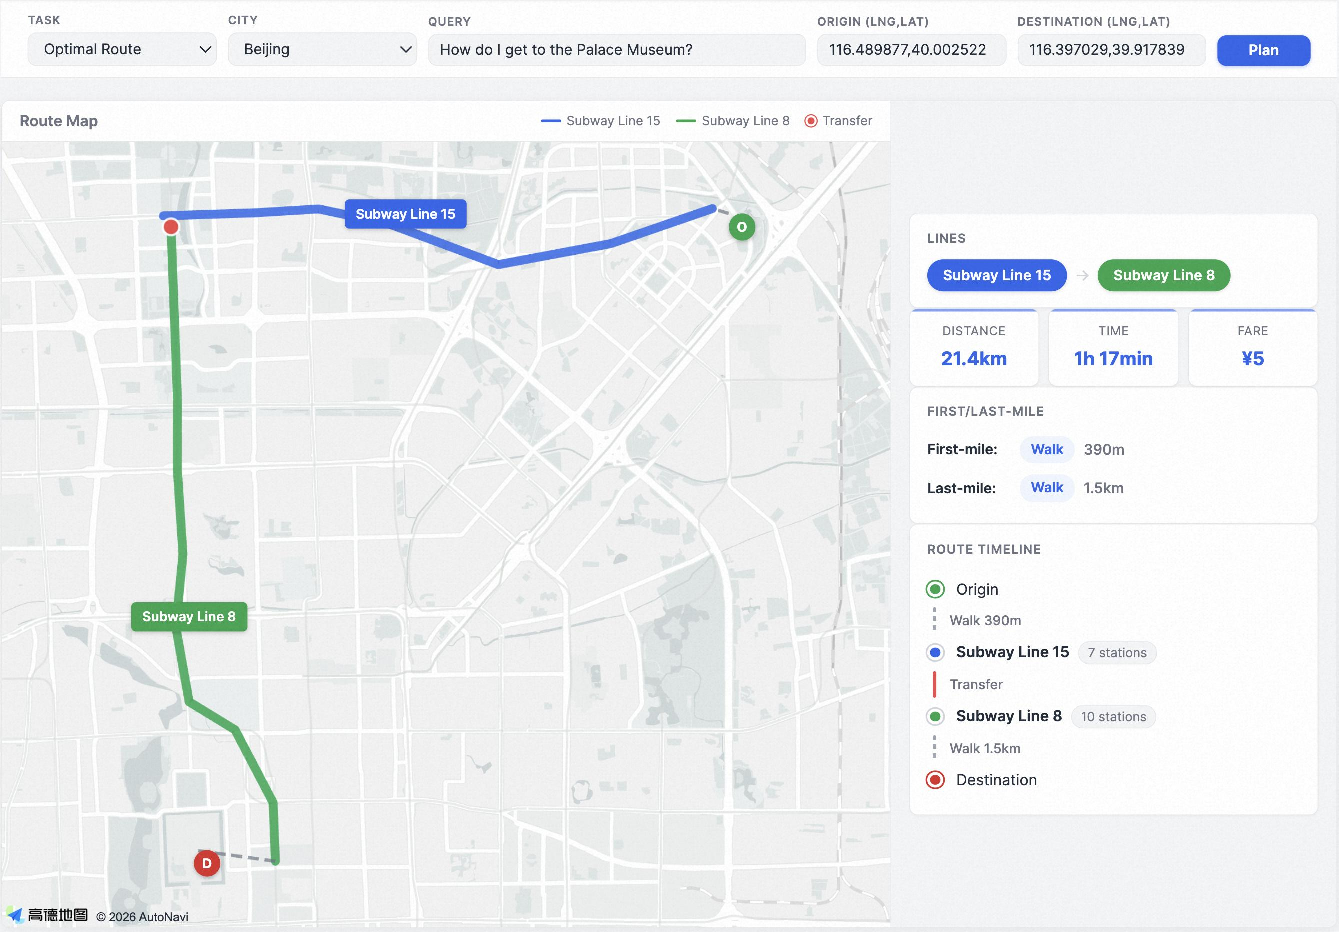
\includegraphics[width=0.96\textwidth]{figures/demo_optimal_route.pdf}
\caption{Optimal Route Generation example from the 4B-Joint model in Beijing. Given a natural-language query and origin--destination coordinates, the model generates a two-segment subway route with transfer, distance, time, fare, and first/last-mile access estimates. The left panel shows the route plotted on a map from station-level GPS coordinates in the model output, and the right panel displays the structured generation.}
\label{fig:demo_optimal}
\end{figure}

\begin{figure}[t]
\centering
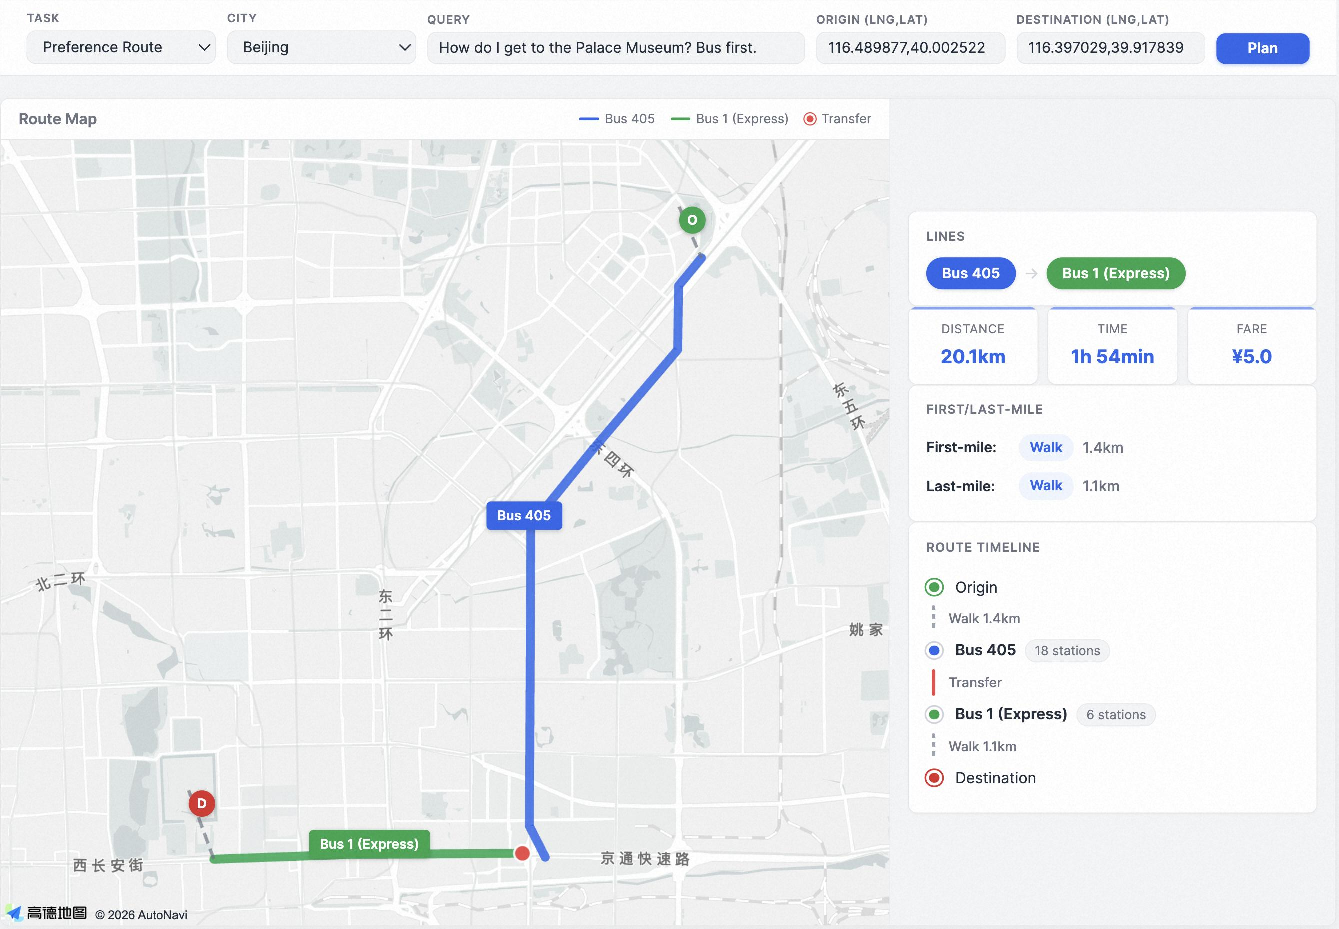
\includegraphics[width=0.96\textwidth]{figures/demo_preference_planning.pdf}
\caption{Preference-Aware Planning example on the same OD pair with an added ``bus first'' constraint. The model avoids all subway segments and generates a bus-only route via Bus~405 and Bus~1~Express, demonstrating preference compliance.}
\label{fig:demo_preference}
\end{figure}

\begin{figure}[t]
\centering
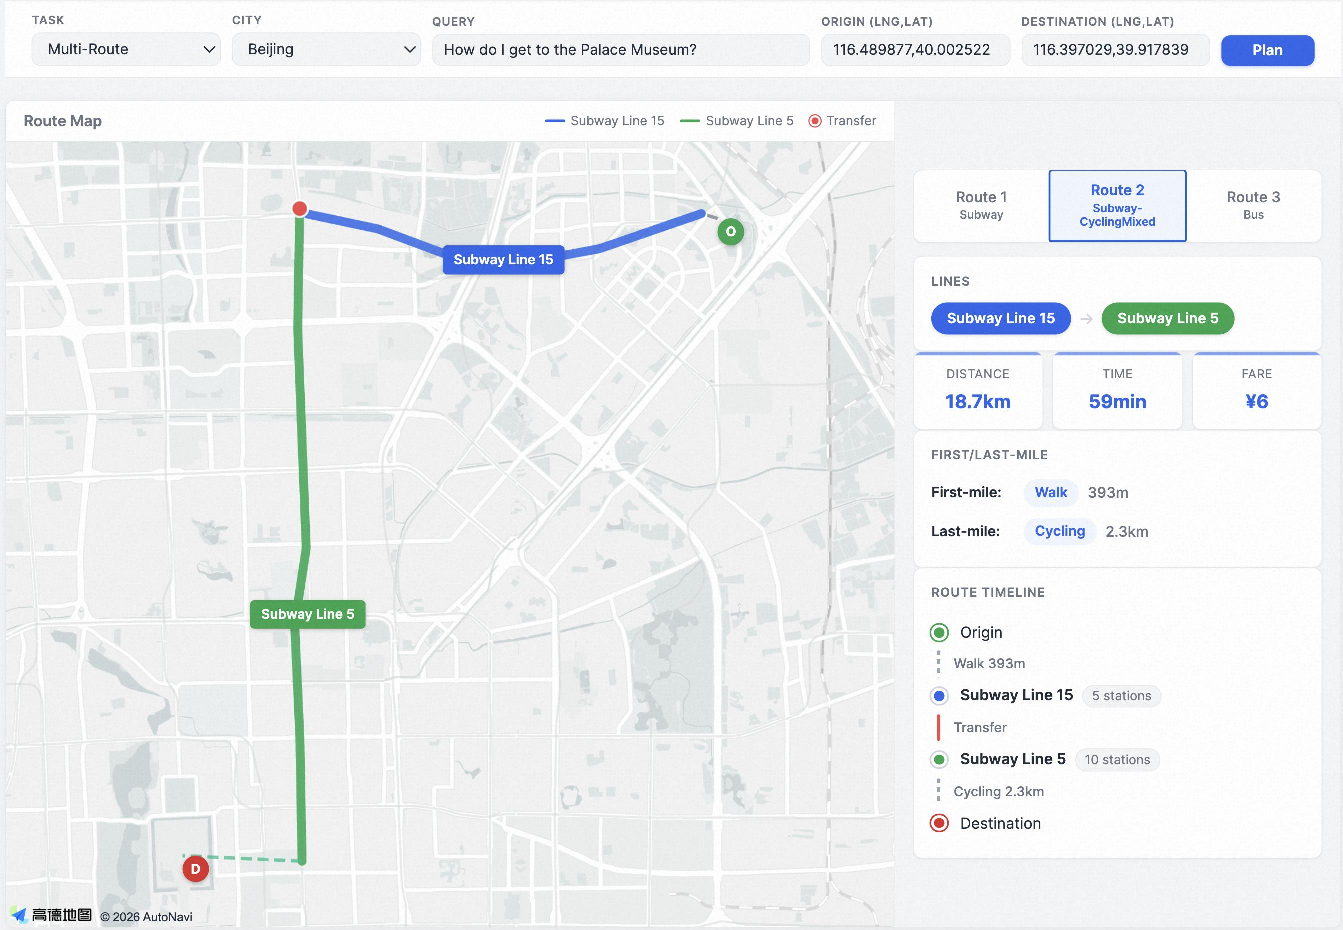
\includegraphics[width=0.96\textwidth]{figures/demo_multi_route.pdf}
\caption{Multi-Route Generation example on the same OD pair. The model produces three alternatives spanning subway, subway with cycling, and bus. Route~2 is visualized due to space constraints.}
\label{fig:demo_multi}
\end{figure}

\begin{figure}[t]
\centering
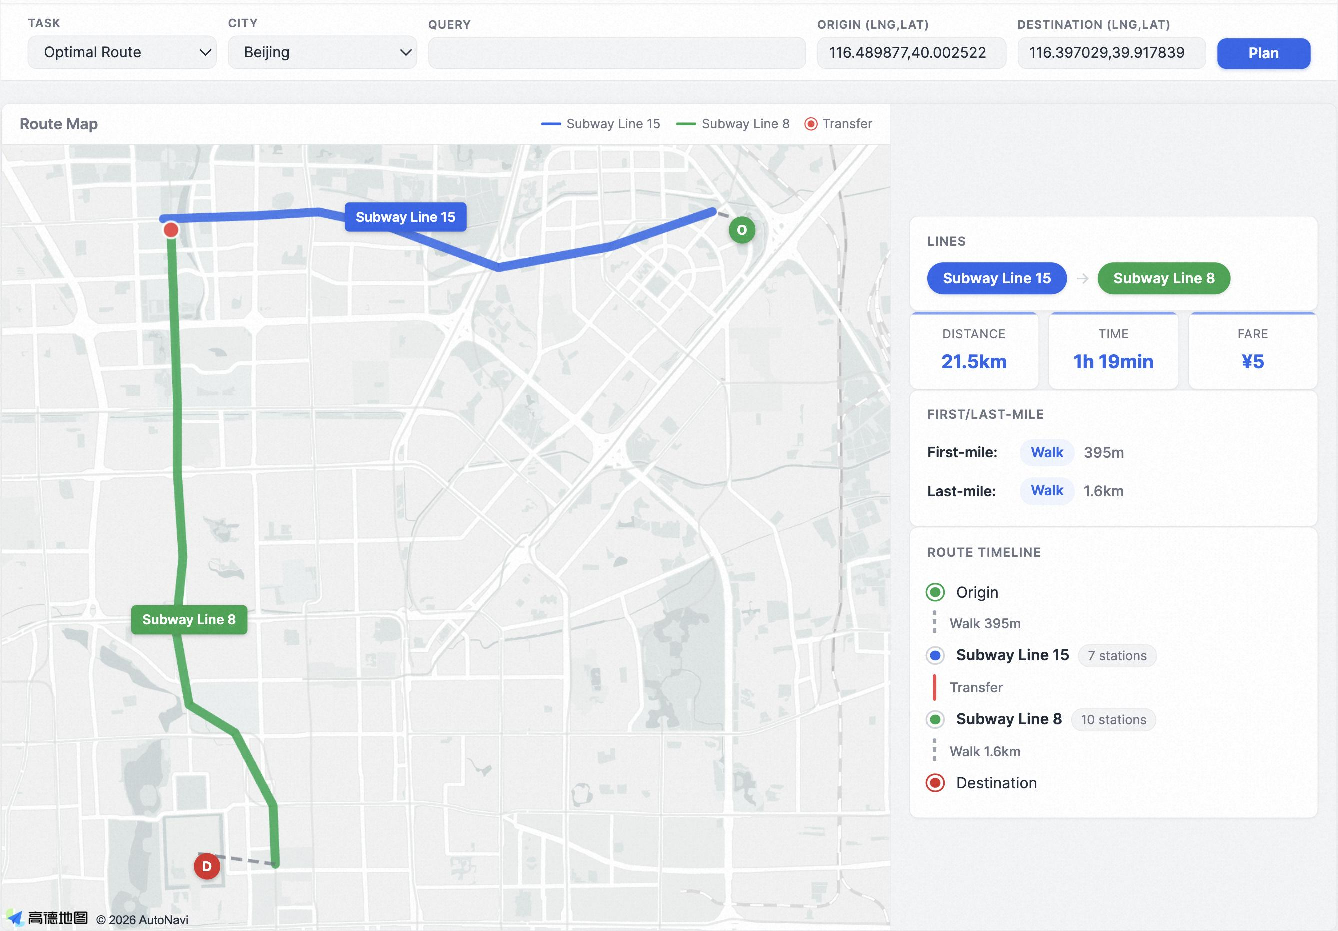
\includegraphics[width=0.96\textwidth]{figures/demo_gps_only_route.pdf}
\caption{GPS-only Optimal Route Generation on the same OD pair with the textual query removed. The generated route is nearly identical to Figure~\ref{fig:demo_optimal}, confirming that spatial grounding is independent of input modality.}
\label{fig:demo_gps}
\end{figure}

\clearpage
% \input{checklist}

\end{document}
